\documentclass[11pt]{article}
\usepackage[a4paper,left=6em,right=6em]{geometry}
\usepackage{amsmath,amsfonts,amsthm,bbold}
\usepackage{booktabs,float,multirow}
\usepackage{cancel}
\usepackage{enumitem}
\usepackage{multicol}
\usepackage{graphicx}
\usepackage[toc,title]{appendix}
\usepackage{tikz}
\usetikzlibrary{
    decorations.pathreplacing,
    decorations.pathmorphing,
    arrows.meta
}
\usepackage{subcaption}
\usepackage{fancyhdr}
\pagestyle{fancy}
\setlength{\headheight}{15pt}
\usepackage{footmisc}
\usepackage{hyperref}
\usepackage{tocloft}
\hypersetup{
    colorlinks=true, %set true if you want colored links
    linkcolor=blue,
    linktoc=all, %set to all if you want both sections and subsections linked
    citecolor=black,
    filecolor=black,
    urlcolor=black
}
\usepackage[UTF8]{ctex}

\setlength{\cftbeforesecskip}{6pt}
\setlength{\parskip}{0.6em}
\renewcommand{\baselinestretch}{1.3}
\setlist{noitemsep,itemindent=1em,topsep=0em,leftmargin=4em,rightmargin=4em}
\setlist[2]{leftmargin=2em}
\newcommand{\divider}{\vspace{-\parskip}\noindent\rule{\linewidth}{0.4pt}}

\newtheorem{thm}{定理}[section] 
\newtheorem{defi}[thm]{定义}
\newtheorem{lemm}[thm]{引理}
\newtheorem{coro}[thm]{推论}

\newcommand{\E}{\mathbb{E}}
\newcommand{\rnE}{\widetilde{\mathbb{E}}}
\newcommand{\wt}[1]{\widetilde{#1}}
\DeclareMathOperator{\Var}{Var}
\DeclareMathOperator{\Cov}{Cov}
\newcommand{\abs}[1]{\left\lvert #1\right\rvert}
\newcommand{\norm}[1]{\left\lVert #1\right\rVert}

\title{随机分析}
\author{杨弘毅}
\date{创建: 2020 年 4 月 19 日 \\修改: \today}

\begin{document}
\maketitle

\tableofcontents

\section{布朗运动与维纳过程}

\textbf{布朗运动}(Brownian motion)指是微小粒子或者颗粒在流体中做无规则运动。在数学中将这种运动定义为\textbf{维纳过程}(Wiener process)是一种连续时间随机过程,为描述证券价格随机性的基本模型,而对于期权以及其他的金融衍生品则可认为是证券价格的函数,此时衍生品价格为证券价格这一随机过程的函数。即只需要假定标的资产遵循的随机过程,利用伊藤引理可得到衍生品遵循随机过程,使得我们可以利用随机分析(Stochastic calculus)这一工具,对期权以及其他金融衍生品的价格进行量化建模。早在1900年法国人路易斯 • 巴舍利耶(Louis Bachelier)在他的博士论文《投机理论》(Théorie de la spéculation)中首次使用随机过程(现称布朗运动)分析股票和期权的价格。比爱因斯坦于1905年提出的描述花粉粒子在水中运动的论文提早了5年。

标准布朗运动(Standard Brownian motion)简易表达式(连续形式)有,其中$\varepsilon \sim N(0,1)$:
\begin{equation*}
    dW_t = \varepsilon_t \sqrt{dt}
\end{equation*}

离散形式有:
\begin{equation*}
    W_T - W_t = \sum^n_{i=1} \varepsilon_i \sqrt{\Delta t}
\end{equation*}

\subsection{特征}

布朗运动或维纳过程,为定义在非负时域t上连续随机过程。虽然连续但其\textbf{处处不可微分},其特征有:
\begin{itemize}
    \item 初值为零
    \item 独立增量:对于任意两个不同时间点$\Delta t_i$与$\Delta t_j$,其增量$\Delta W_i$与$\Delta W_j$相互独立
    \item 平稳性:增量$\Delta W$服从均值为零、方差等于时间长度的正态分布,即$\Delta W_i \sim N(0,\Delta t_i)$
\end{itemize}

并且由如上性质可知,布朗运动是一个马尔科夫过程(Markov process),即该过程在任意t时刻之后的位置,仅和t时刻的位置有关,与之前的历史轨迹无关。即该过程的当前值就包含了对其未来做预测所需的全部信息。并且由于其虽然连续,但处处不可微分的性质,使得几个点微积分无法使用,只能使用伊藤微积分(Itô calculus)进行运算。

\subsection{部分证明}

\textbf{增量均值为零,方差为时间长度},当$X$与$Y$独立时,则有:
\begin{equation*}
    \Var(XY) = \Var(X)\Var(Y) + [\E(X)]^2 \Var(Y) + [E(Y)]^2 \Var(X)
\end{equation*}

此时,由于$\varepsilon_t$与$dt$独立,套用上式,同时由于$\varepsilon_t \sim N(0,1)$,则有:
\begin{equation*}
    \E(dZ_t) = \E(\varepsilon_t \sqrt{dt}) = 0
\end{equation*}

应为方差有:
\begin{align*}
    \Var(dZ_t) & = \Var( \varepsilon_t \sqrt{dt}) \\
    & =  \Var(\varepsilon_t) \Var(\sqrt{dt}) + [\E(\varepsilon_t)]^2 \Var(\sqrt{dt}) + [E(\sqrt{dt})]^2 \Var(\varepsilon_t) \\
    & = \Var(\varepsilon_t) \left[ \Var[(\sqrt{dt})^2] - [\E(\sqrt{dt})]^2 \right] \\
    & = \Var(\varepsilon_t) \left[ \E[(\sqrt{dt})^2] - [\E(\sqrt{dt})]^2 + [\E(\sqrt{dt})]^2 \right] \\
    & = 1 \cdot \E(dt) = dt
\end{align*}

\textbf{方差可加性},由下式可见,由于独立增量,导致协方差项为零,使得方差可加。
\begin{align*}
     & \Var(X_1+X_2+X_3) \\
     & = \Var(X_1) + \Var(X_2) + \Var(X_3) \\
     & + \Cov(X_1,X_2) + \Cov(X_2,X_3) + \Cov(X_1,X_3)
\end{align*}

由上可知,增量在连续形式$dW_t$以及离散形式$W_T-W_t$下,均服从均值为零,方差为时间长度的正态分布,即有:
\begin{align*}
    dW_t & \sim N(0,dt) \\
    W_T - W_t & \sim N(0,T-t)
\end{align*}

\subsection{二次变差}

考虑区间$[0,T]$,定义$\Pi=\{0=t_0<t_1<t_2<\dots<t_N=T\}$和最大步幅$\norm{\Pi} = \max\limits_{i}(t_{i+1}-t_{i})$。为方便后续推导,假设步幅相同,即$t_{i+1} - t_{i} = \tfrac{T}{n}$。$s_i \in (t_i,t_{i+1})$,则有对于任意一个连续函数$f(t)$,其二次变差(Quadratic variation)定义为:
\begin{equation*}
    \sum^{N-1}_{i=0} \left[ f(t_{i+1} - f(t_i)) \right]^2
\end{equation*}

对于一个连续且在$[0,T]$中处处可微的函数$f(t)$,$t_{i^*} \in [t_{i},t_{i+1}]$,利用微分中值定理,可以看到随着时间的越来越细的划分,$\norm{\Pi}$趋近于零。则可得到处处可微的连续函数,在区间$[0,T]$的二次变分为0。
\begin{align*}
    \sum_{i=0}^{N-1} \left[ f(t_{i+1}) -f(t_{i}) \right]^2 
    &= \sum_{i=0}^{N-1} f'(t_{i^*})^2 (t_{i+1} - t_{i})^2 \\
    &= \norm{\Pi} \sum_{i=0}^{N-1} f'(t_{i^*})^2 (t_{i+1} - t_{i})
\end{align*}

于是有:
\begin{align*}
    [f,f](T) &= \lim\limits_{\norm{\Pi} \rightarrow 0} \norm{\Pi} \left[ \sum_{i=0}^{N-1} f'(t_{i^*})^2 (t_{i+1} - t_{i}) \right] \\
    &= \lim\limits_{\norm{\Pi} \rightarrow 0} \norm{\Pi} \cdot \lim\limits_{\norm{\Pi} \rightarrow 0} \sum_{i=0}^{N-1} f'(t_{i^*})^2 (t_{i+1} - t_{i}) \\
    &= \lim\limits_{\norm{\Pi} \rightarrow 0} \norm{\Pi} \cdot \int^T_0 f'(t_{i^*})^2 dt = 0
\end{align*}

证明需要假设$\int^T_0 f'(t_{i^*})^2 dt$为有限,如果为无限则会出现$0\cdot \infty$的情形。

\begin{thm}
    设$\Pi=\{0=t_0<t_1<t_2<\dots<t_N=T\}$为$[0,T]$的分划。布朗运动对应的样本二次变差有:
    \begin{align*}
        Q_{\Pi} = \sum_{i=0}^{N-1} \left[ W(t_{i+1}) - W(t_{i}) \right]^2 = T \qquad \text{almost surely.}
    \end{align*}
\end{thm}

\begin{proof}
    样本二次变差为独立随机变量所组成,因此其均值为这些随机变量的均值,方差为这些随机变量方差之和。并且有$\Var X = \E X^2 - \E^2 X $:
    \begin{equation*}
        \E [(W(t_{i+1}) - W(t_{i}))^2] = \Var [W(t_{i+1}) - W(t_{i})] + \E^2 [W(t_{i+1}) - W(t_{i})]= t_{i+1} - t_{i}
    \end{equation*}

    由此可以得到:
    \begin{equation*}
        \lim\limits_{\norm{\Pi} \rightarrow 0} \E(Q_{\Pi})
        = \sum_{i=0}^{N-1} \E \left[(W(t_{i+1}) - W(t_{i}))^2 \right]
        =  \sum_{i=0}^{N-1} (t_{i+1} - t_{i}) = T
    \end{equation*}

    对于方差,应有:
    \begin{equation*}
        \Var [(W(t_{i+1}) - W(t_{i}))^2] = \E [(W(t_{i+1}) - W(t_{i}))^4] - \E^2 [(W(t_{i+1}) - W(t_{i}))^2]
    \end{equation*}

    对于四次方项$\E [(W(t_{i+1}) - W(t_{i}))^4]$,可通过对正态分布矩母函数$M_X(t)$对$t$不断求导得到其期望,需求四阶导数$M_X^{(4)}(t)$:
    \begin{align*}
        M_X(t) &= \E(e^{xt}) = e^{\mu t + \frac{1}{2} \sigma^2 t^2} \\
        M'_X(t) &= (\mu + \sigma^2 t)e^{\mu t + \frac{1}{2} \sigma^2 t^2} \\
        M''_X(t) &= (\mu^2 + 2 \mu \sigma^2 t + \sigma^4 t^2 + \sigma^2)e^{\mu t +\frac{1}{2} \sigma^2 t^2} \\
        M^{(3)}_X(t) &= (\mu^3 + 3 \mu^2 \sigma^2 t + 3\mu \sigma^4 t^2 + 3\mu \sigma^2 + \sigma^6 t^3 + 3\sigma^4 t)e^{\mu t +\frac{1}{2} \sigma^2 t^2} \\
        M^{(4)}_X(t) &= (\mu^4 + 4 \mu^3 \sigma^2 t + 6 \mu^2 \sigma^4 t^2 + 6\mu^2 \sigma^2 + 4\mu\sigma^6 t^3 \\
        &\qquad + 12\mu\sigma^4 t + \sigma^8 t^4 + 6\sigma^6 t^2 + 3\sigma^4)e^{\mu t +\frac{1}{2} \sigma^2 t^2}
    \end{align*}

    因为$W(t_{i+1}) - W(t_{i}) \sim N(0,t_{i+1}-t_{i})$,其均值$\mu=0$计算四阶中心矩$M_X^{(4)}(0) = 3\sigma^2$,令$t=0$:
    \begin{equation*}
        \E [(W(t_{i+1}) - W(t_{i}))^4] = 3(t_{i+1}-t_{i})^2 
    \end{equation*}

    因此可继续计算单个时间间隔的方差:
    \begin{align*}
        \Var [(W(t_{i+1}) - W(t_{i}))^2] &= \E [(W(t_{i+1}) - W(t_{i}))^4] - \E^2 [(W(t_{i+1}) - W(t_{i}))^2] \\
        &= 3(t_{i+1}-t_{i})^2 - (t_{i+1}-t_{i})^2 \\
        &= 2(t_{i+1}-t_{i})^2
    \end{align*}

    因此在$[0,T]$的方差为:
    \begin{align*}
        \Var(Q_{\Pi}) &= \sum_{i=0}^{N-1} \Var \left[(W(t_{i+1}) - W(t_{i}))^2 \right] \\
        &=  \sum_{i=0}^{N-1} 2(t_{i+1}-t_{i})^2
        \leq \sum_{i=0}^{N-1} 2\norm{\Pi} (t_{i+1}-t_{i}) \\
        &= 2\norm{\Pi} \sum_{i=0}^{N-1} (t_{i+1}-t_{i}) \\
        &= 2\norm{\Pi} T
    \end{align*}

    由此可知当最大步幅$\norm{\Pi}$趋近于零时,方差也将趋近于零:
    \begin{align*}
        \lim\limits_{\norm{\Pi} \rightarrow 0} \Var(Q_{\Pi}) = 0
    \end{align*}

    利用切比雪夫不等式(Chebyshev's inequality):
    \begin{align*}
        P\left( \abs{Q_{\Pi} - \E(Q_{\Pi}} \geq \frac{1}{n} \right) &\leq n^2 \Var(Q_{\Pi}) \\
        \lim_{\norm{\Pi} \rightarrow 0} P\left( \abs{Q_{\Pi} - T} \geq \frac{1}{n} \right) &\leq n^2 \lim_{\norm{\Pi} \rightarrow 0} \Var(Q_{\Pi})  \\
        \lim_{\norm{\Pi} \rightarrow 0} P\left( \abs{Q_{\Pi} - T} \geq \frac{1}{n} \right) &= 0
    \end{align*}
    
    因此在概率上几乎必然成立,即虽然有可能存在某些布朗运动使得其二次变差为T不成立,但这样的情形概率为0:
    \begin{equation*}
        \lim_{\norm{\Pi} \rightarrow 0} Q_{\Pi} = \E Q_\Pi = T
    \end{equation*}
\end{proof}

可以看到而对于布朗运动$B(t)$,虽然连续但处处不可微分,使得其无法像其他连续可微分函数一样计算二次变差。其非零的二次变分说明随机性使得它的波动太频繁,以至于不管我们如何细分区间、得到多么微小的划分区间T,累加这些微小区间上的变化总和,二次变分都不会消失(即二次变分不为0),而是等于这个区间的长度T。布朗运动的二次变差可简写为无穷小量,为$(dB)^2=dt$。其中无穷小量在英文中应为differential或infinitesimal difference,其中infinitesimal即infinitely small。

\subsection{几种随机过程}

\textbf{广义维纳过程}(generalized Wiener process),a与b为常数。此时,易知其均值为$\E(dX_t) = adt$,由于$b$为常数,且$\Var(dW_t)=dt$,则有方差为$\Var(dX_t)=b^2 dt$。
\begin{equation*}
    dX_t = a dt + b dW_t
\end{equation*}

\textbf{普通布朗运动},a(t)与b(t)都是t的确定性函数。由于都为确定函数,所以如上可知,其均值方差为$\E(dX_t) = a(t)dt$,由于$b$为常数,且$\Var(dW_t)=dt$,则有方差为$\Var(dX_t)=b(t)^2 dt$。
\begin{equation*}
    dX_t = a(t) dt + b(t) dW_t
\end{equation*}

\textbf{伊藤扩散过程}(Itô diffusion),此时$a(X(t),t)$与$b(X(t),t)$都为$X_t$和$t$的确定性函数。由于漂移项与方差项都包含$X(t)$,使得扩散之后过程的条件分布无法保证仍是正态分布。但更能刻画一般动态变化,未加入新的风险源,仍具有独立增量,马尔可夫性,和方差可加性等性质。
\begin{equation*}
    dX_t =a(X(t),t) dt + b(X(t),t) dW_t
\end{equation*}

以上都为\textbf{随机微分方程}(Stochastic differential equation,SDE),与普通微分方程的延伸,特指的是包含随机过程的微分方程。\textbf{注意}:虽然$B(t)$处处不可微,单$dB(t)$指布朗运动在一个无限小的时间间隔内的变化。

\section{伊藤引理}

\subsection{古典微积分为何失效}

有了随机过程$X_t$或维纳过程$W_t$,由于衍生品价格是标的资产价格$S_t$与时间$t$的函数。我们就需要进一步研究随机过程的函数,研究$f$在无穷小的时间间隔内的变化,即$df(\cdot)$。由上在分析二次变差可以发现,由于布朗运动处处不可微的性质,使得古典微积分无法适用于随机过程。日本数学家伊藤清(Itō Kiyoshi)提出伊藤微积分解决了这一问题。

对于古典的微积分中的链式法则,由于布朗运动处处不可微分,即$dW_t/dt$不存在,使得等式无意义。
\begin{equation*}
    \frac{df(W_t)}{dt} = f'(W_t)\frac{dW_t}{dt}
\end{equation*}

对于函数$f(x)$使用泰勒展开,应有:
\begin{equation*}
    f(x + \Delta x) - f(x)= f'(x)(\Delta x) + \frac{1}{2} f''(x)(\Delta x)^2 + \frac{1}{6} f'''(x)(\Delta x)^3 + \dots
\end{equation*}

对于普通变量$X$,可以发现当$\Delta x$趋近于$0$时,除了第一项,其他项都为高阶小量,因此均可被忽略,因此其无穷小量形式应为$df=f'(x)dx$。而对于随机变量$W_t$,进行泰勒展开:
\begin{equation*}
    df = f(W_t + \Delta W_t) - f(W_t)= f'(W_t)(\Delta W_t) + \frac{1}{2} f''(W_t)(\Delta W_t)^2 + \frac{1}{6} f'''(W_t)(\Delta W_t)^3 + \dots
\end{equation*}

与普通随机变量相同的是第一项需要保留,但第二项对于普通随机变量来说已经是高阶小量了,但对于随机过程变量$W_t$,已知其二次变差为$(dW_t)^2 = dt$,与第一项为同阶,不能忽略。而从第三项开始之后的所有项才可以被忽略,因此得到伊藤引理的最基本形式:
\begin{equation*}
    df(W_t) =f'(W_t)dW_t + \frac{1}{2}f''(W_t)dt
\end{equation*}

\subsection{伊藤引理与证明}

\begin{lemm}
    伊藤引理(Itô lemma),假设变量$X_t$遵循如下随机过程:
    \begin{equation*}
        dX_t =\mu_t dt + \sigma_t dW_t
    \end{equation*}

    在导数$\dfrac{\partial f}{\partial t}$、$\dfrac{\partial f}{\partial X}$与$\dfrac{\partial^2 f}{\partial X^2}$存在的前提下,则有变量$X_t$和$t$的函数$f(X(t),t)$将遵循如下过程:
    \begin{equation*}
        df(X_t,t) = \left(\frac{\partial f}{\partial t} + \mu_t \frac{\partial f}{\partial x} + \frac{1}{2} \sigma_t^2 \frac{\partial^2 f}{\partial x^2} \right)dt + \sigma_t \frac{\partial f}{\partial X} dW_t
    \end{equation*}
\end{lemm}

\begin{proof}
    $f(X,t)$的泰勒展开式为:
    \begin{equation*}
        \Delta f_t = \frac{\partial f}{\partial X} \Delta X + \frac{\partial f}{\partial t} \Delta t + \frac{1}{2} \frac{\partial^2 f}{\partial X^2}\Delta X^2  + \frac{\partial f}{\partial X \partial t}\Delta X \Delta t + \frac{1}{2} \frac{\partial^2 f}{\partial t^2} \Delta t^2 + \dots
    \end{equation*}

    当$\Delta t \rightarrow 0$时,$(\Delta t)^2$,认为是高阶无穷小,可忽略。而对于$\Delta X \Delta t$项有:
    \begin{align*}
        \Delta X &= a\Delta t + b \varepsilon\sqrt{\Delta t} \\
        \Delta X \Delta t &= a(\Delta t)^2 + b \varepsilon(\Delta t)^{3/2}
    \end{align*}

    其中的$(\Delta t)^{3/2}$项,也被认为时高阶无穷小项,可忽略。同时由于$(\Delta X)^2$项中包含$\Delta t$项,因此需要保留。仅考虑前三项,展开得到:
    \begin{align*}
        \Delta f_t & = \frac{\partial f}{\partial X} \Delta X + \frac{\partial f}{\partial t} \Delta t + \frac{1}{2} \frac{\partial^2 f}{\partial X^2}\Delta X^2 \\
        & = \frac{\partial f}{\partial X} \Delta X + \frac{\partial f}{\partial t} \Delta t + \frac{1}{2} \frac{\partial^2 f}{\partial X^2} [a\Delta t + b\varepsilon\sqrt{\Delta t}]^2 \\
        & = \frac{\partial f}{\partial X} \Delta X + \frac{\partial f}{\partial t} \Delta t + \frac{1}{2} \frac{\partial^2 f}{\partial X^2} b^2 \varepsilon^2 \Delta t
    \end{align*}

    对于$\varepsilon^2 \Delta t$项,由于$\varepsilon \sim N(0,1)$,因此有$\E(\varepsilon)=0$。又因$\Var(\varepsilon)=\E(\varepsilon^2)-[\E(\varepsilon)]^2=1$,得到$\E(\varepsilon^2)=1$,同时有$\E(\varepsilon^2 \Delta t) = \Delta t$。计算$\varepsilon^2 \Delta t$的方差可得:
    \begin{align*}
        \Var(\varepsilon^2 \Delta t) & = \Var(\varepsilon^2) \Var(\Delta t) + [\E(\varepsilon^2)]^2 \Var(\Delta t) + [E(\Delta t)]^2 \Var(\varepsilon^2) \\
        & = \Var(\varepsilon^2) \Var(\Delta t) + 1 \cdot \Var(\Delta t) + [E(\Delta t)]^2 \Var(\varepsilon_t^2) \\
        & = \mathcal{O}(\Delta t^2)
    \end{align*}

    可以认为$\varepsilon^2 \Delta t$方差为高阶无穷小,其期望为$1$。因此,可认为$\varepsilon^2 \Delta t \approx \Delta t$,可将原式化简为:
    \begin{equation*}
        \Delta f_t = \frac{\partial f}{\partial X} \Delta X + \frac{\partial f}{\partial t} \Delta t + \frac{1}{2} \frac{\partial^2 f}{\partial X^2} b^2 \Delta t
    \end{equation*}

    而连续形式为:
    \begin{align*}
        df_t & = \frac{\partial f}{\partial X}  dX_t + \frac{\partial f}{\partial t} dt + \frac{1}{2} \frac{\partial^2 f}{\partial X^2} b^2 dt \\
        & = \frac{\partial f}{\partial X} (a_t dt + b_t dW_t) + \frac{\partial f}{\partial t} dt + \frac{1}{2} \frac{\partial^2 f}{\partial X^2} b^2 dt \\
        & = \left(\frac{\partial f}{\partial X}a_t  + \frac{\partial f}{\partial t} + \frac{1}{2}\frac{\partial^2 f}{\partial X^2} b^2_t \right)dt + \frac{\partial f}{\partial X} b_t dW_t
    \end{align*}
\end{proof}

由此可知,$f$作为随机过程$X$与时间$t$的函数,其本身也是一个随机过程。而$df_t$与$dX_t$的随机性\textbf{来源于同一布朗运动}$dW_t$,而非两个独立的布朗运动。为方便记忆,可记为(金融随机分析第二卷 P118):
\begin{equation*}
    \boxed{
        df(X(t),t) = f_t(X(t),t)dt + f_x(X(t),t)dX(t) + \frac{1}{2}f_{xx}(X(t),t)dX(t)dX(t)
    }
\end{equation*}

或可写为更简洁的形式:
\begin{equation*}
    \boxed{
        df = f_t dt + f_x dX + \frac{1}{2}f_{xx}dXdX
    }
\end{equation*}

\section{几何布朗运动}

由上可知随机过程$X(t)$随着时间$t$的变化,可能为负数,但股票价格显然不可能为负。收益率却有正有负,因此可以使用$X(t)$来描绘收益率。假设$S_t$为股票价格,可以假设其百分比收益率遵循如下随机过程:
\begin{equation*}
    \frac{dS_t}{S_t} = \mu dt + \sigma dW_t
\end{equation*}

因此$S_t$的随机微分形式如下,此时股票价格$S_t$服从\textbf{几何布朗运动}(Geometric Brownian Motion,GBM):
\begin{equation*}
    dS_t = \mu S_t dt + \sigma S_t dW_t
\end{equation*}

令$f(S_t) = \ln S_t$,此时:
\begin{equation*}
    \frac{\partial f}{\partial S} = \frac{1}{S_t}, \quad
    \frac{\partial^2 f}{\partial S^2} = -\frac{1}{S_t^2}, \quad
    \frac{\partial f}{\partial t} = 0
\end{equation*}

代入伊藤引理之中,此时$a_t=\mu S_t$,$b_t=\sigma S_t$,则有:
\begin{align*}
    df_t = d \ln S_t & = \left( \frac{1}{S_t}\mu S_t + 0 - \frac{1}{2} \frac{1}{S_t^2} \sigma^2 S_t^2 \right) dt + \frac{1}{S_t}\sigma S_t dW_t \\
    & = \left( \mu - \frac{1}{2}\sigma^2\right)dt + \sigma dW_t
\end{align*}

连续形式下有:
\begin{equation*}
    d\ln S = \left( \mu - \frac{1}{2}\sigma^2\right) dt + \sigma dW_t \sim N \left( (\mu-\frac{\sigma^2}{2})dt, \sigma^2 dt \right)
\end{equation*}

离散形式下为:
\begin{align*}
    \Delta \ln S &= \ln S_T - \ln S_t = \left( \mu - \frac{\sigma^2}{2} \right) \Delta t + \sigma (W_T - W_t) \\
    \Delta \ln S &\sim N \left((\mu-\frac{\sigma^2}{2})(T-t), \sigma^2(T-t) \right)
\end{align*}

可以看到\textbf{连续复利收益率}或\textbf{对数收益率}服从期望值为$(\mu - \tfrac{\sigma^2}{2})dt$,方差为$\sigma^2 dt$的\textbf{正态分布},与现实较为吻合。且$d\ln S_t$的定义,使得股票价格非负。对于日频收益率的计算,此时得到的正态分布均值以及方差均为日频($T-t=\frac{1}{252}$),需乘以252进行年化,得到年化的收益率均值与波动率。在$T$时刻,\textbf{股票价格的对数}($\ln S$),也服从\textbf{正态分布},则有\textbf{股票价格}($S$)服从\textbf{对数正态分布}。
\begin{equation*}
    \ln S_T  \sim N \left(\ln S_t + (\mu-\frac{\sigma^2}{2})(T-t), \sigma^2(T-t)\right)
\end{equation*}

可以看到选择几何布朗运动描绘股票价格$S_t$有如下几大优点:
\begin{itemize}[leftmargin=4em]
    \item 正态分布:经验事实证明,股票价格的连续复利收益率,近似地服从正态分布
    \item 马尔科夫过程:由布朗运动的性质可知,利用几何布朗运动描绘的股票价格是一个马尔科夫过程,即当前价格就包含了对其未来做预测所需的全部信息,这与弱有效市场假说相符
    \item 布朗运动在时间上处处不可微以及二次变分不为零的性质符合股票收益率在时间上存在转折尖点的特征。
\end{itemize}

\section{对数正态分布}

由\textbf{股票价格的对数}服从\textbf{正态分布}可知,股票价格应服从\textbf{对数正态分布}(Log-normal distribution)。由正态分布与对数正态分布的性质可知,对一个服从正态分布的随机变量$X$取指数,则$e^X$服从对数正态分布。相反,对一个服从对数正态分布的随机变量$X$取对数,则$\ln X$服从正态分布(因而得名,取对数得到正态分布的分布)。因此有如下关系:
\begin{align*}
    \ln S_T \sim N(\mu,\sigma^2) \quad \leftrightarrow \quad S_T \sim \text{Log-normal}(\mu,\sigma^2)
\end{align*}

对于对数正态分布$X \sim \text{Log-normal}(\mu,\sigma^2)$,其期望与标准差为:
\begin{align*}
    \E(X) & = e^{\mu+\frac{\sigma^2}{2}} \\
    \Var(X) & = e^{2\mu+\sigma^2} (e^{\sigma^2}-1)
\end{align*}

已知股票价格的对数$\ln S_T$服从如下正态分布:
\begin{equation*}
    \ln S_T  \sim N \left(\ln S_t + (\mu-\frac{\sigma^2}{2})(T-t), \sigma^2(T-t)\right)
\end{equation*}

那么股票价格$S_T$服从如下对数正态分布:
\begin{equation*}
    S_T  \sim \text{Log-normal} \left(\ln S_t + (\mu-\frac{\sigma^2}{2})(T-t), \sigma^2(T-t)\right)
\end{equation*}

可求得股票价格得期望与方差为:
\begin{align*}
    \E(S_T)   & = \exp\left( \ln S_t + (\mu - \frac{\sigma^2}{2})(T-t)+\frac{\sigma^2(T-t)}{2}\right) \\
    & = \exp \left( \ln S_t + \mu(T-t) \right) \\
    & = S_t e^{\mu(T-t)} \\
    \Var(S_T) & = \left[\exp(\sigma^2(T-t))-1\right] \exp \left\{2\left[\ln S_t + (\mu - \frac{\sigma^2}{2})(T-t)\right] + \sigma^2(T-t)\right\} \\
    & = \left[\exp(\sigma^2(T-t))-1\right] \exp\left[2 \ln S_t + 2\mu (T-t)\right] \\
    & = S_t^2 e^{2\mu(T-t)} \left[ e^{\sigma^2 (T-t)} - 1 \right]
\end{align*}

\subsection*{注意}

对于正态分布$\mu$与$\sigma^2$,为其均值与标准差。而对于对数正态分布,仅为确定其分布的两个参数。对于相同的$\mu$与$\sigma$参数确定的正态分布与对数正态分布,两者之间的期望与方差通过如下表格关系转化:
\begin{table}[H]
\centering
\begin{tabular}{@{}cll@{}}
\toprule
\multicolumn{1}{l}{}
& \multicolumn{1}{c}{\textbf{正态分布}} & \multicolumn{1}{c}{\textbf{对数正态分布}} \\
\midrule
\multirow{1}{*}{\textbf{期望}} 
& $\E_N(X) \equiv \mu = \ln[\E_{L}(X)] - \frac{1}{2} \ln \left[1+\frac{\Var_{L}(X)}{[\E_{L}(X)]^2}\right] $ & $\E_{L}(X) = e^{\mu+\frac{1}{2}\sigma^2}$ \\
\textbf{方差} & $\Var_N(X) \equiv \sigma^2 = \ln \left[1+\frac{\Var_{L}(X)}{[\E_{L}(X)]^2}\right]$ & $\Var_{L}(X) = e^{2\mu+\sigma^2} 
\left(e^{\sigma^2} - 1\right)$ \\
\bottomrule
\end{tabular}
\end{table}

\subsection{PDF与CDF}

如下图所示,通过对服从\textbf{正态分布}的随机变量\textbf{取指数},可以将其转换为对数正态分布。同理,通过对服从\textbf{对数正态分布}的随机变量\textbf{取对数},使其转换为正态分布。假设随机变量$Y \sim N(\mu,\sigma^2)$ 服从正态分布,随机变量$X \sim \text{Log}N(\mu,\sigma^2)$,对正态分布随机变量$Y$取指数$x=e^y$,此时有$y = \ln x$,带入CDF中,可得到对数正态函数CDF。对两者求导,可得PDF函数。
\begin{table}[H]
\centering
\begin{tabular}{@{}cll@{}}
\toprule
\multicolumn{1}{l}{}
& \multicolumn{1}{c}{\textbf{正态分布}} & \multicolumn{1}{c}{\textbf{对数正态分布}} \\
\midrule
\multirow{1}{*}{\textbf{PDF}} 
& $\frac{1}{\sigma\sqrt{2\pi}} e^{-\frac{1}{2} \left( \frac{x-\mu}{\sigma} \right)^2 } $
& $\frac{1}{x\sigma\sqrt{2\pi}} e^{-\frac{1}{2} \left( \frac{\ln x-\mu}{\sigma} \right)^2 } $ \\
\textbf{CDF} 
& $\frac{1}{2} \left[1 + \text{erf}\left( \frac{x-\mu}{\sigma\sqrt{2}}\right) \right]$
& $\frac{1}{2} \left[1 + \text{erf}\left( \frac{\ln x-\mu}{\sigma\sqrt{2}}\right) \right]$ \\
\bottomrule
\end{tabular}
\end{table}

\begin{figure}[ht!]
    \centering
    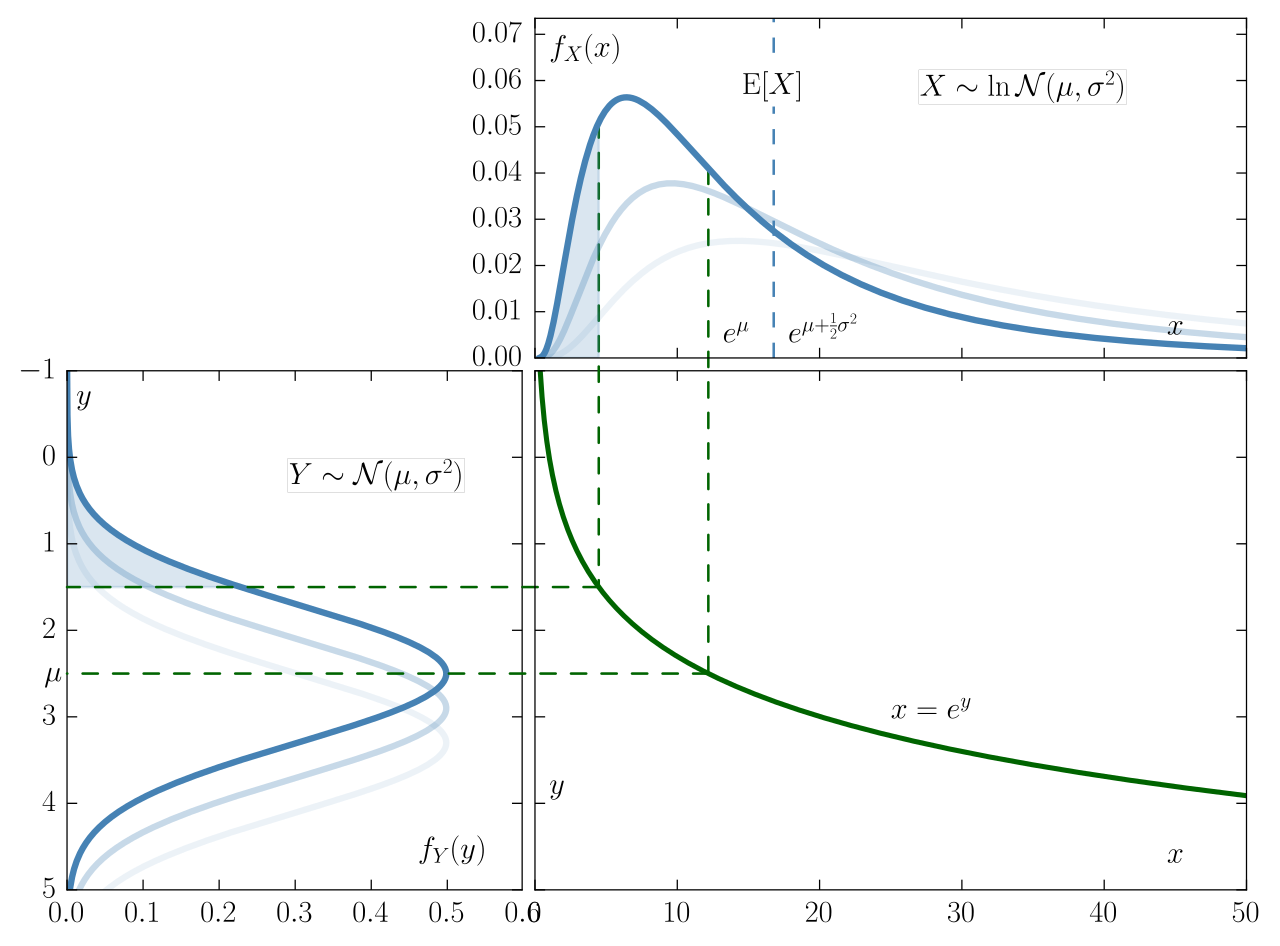
\includegraphics[width=0.9\textwidth]{fig/lognormal-distribution.png}
    \caption{两者相互转换}
    \label{fig:lognormal}
\end{figure}

\subsection{PDF推导}

如上文所述,对于相同参数$\mu$与$\sigma^2$的正态分布与对数正态分布可以相互转化。两者互相经过转化后,其累积分布函数(Cumulative distribution fuction,CDF)相同。如图\ref{fig:lognormal}所示,假设随机变量$Y \sim N(\mu,\sigma^2)$ 服从正态分布,随机变量$X \sim \text{Log}N(\mu,\sigma^2)$,则应有如下关系,对服从对数正态分布的随机变量$X$取对数,使其转化为正态分布:
\begin{equation*}
    \text{CDF}_{logN}(x) = \text{CDF}_N (\ln x) = \text{CDF}_N (y)
\end{equation*}

对公式两边取导数,则可得到其概率密度函数(Probability density function,PDF):
\begin{equation*}
    \text{PDF}_{logN}(x) = \frac{1}{y} \text{PDF}_N(\ln x)
\end{equation*}

此时,带入已知正态分布PDF,即可得到对数正态分布PDF:
\begin{equation*}
    \text{PDF}_{logN} = \frac{1}{x\sigma\sqrt{2\pi}} e^{-\frac{(\ln x - \mu)^2}{2\sigma^2}}
\end{equation*}

\subsubsection{期望推导}

根据对数正态分布的PDF,可计算其期望:
\begin{equation*}
    \E(X) = \int^{+\infty}_0 x f(x) dx = \int^{+\infty}_0 \frac{1}{\sigma\sqrt{2\pi}} e^{-\frac{(ln x - \mu)^2}{2\sigma^2}} dx
\end{equation*}

使用换元法,令$t = \frac{\ln x - \mu}{\sqrt{2}\sigma}$,则有$x = e^{\sqrt{2}\sigma t + \mu}$,则原积分转化为:
\begin{align*}
    \E(X) &= \int^{+\infty}_{-\infty} \frac{1}{\sigma\sqrt{2\pi}}e^{-t^2}d e^{\sqrt{2}\sigma t + \mu}\\ 
    &= \frac{e^{\mu + \frac{\sigma^2}{2}}}{\sqrt{\pi}} \int^{+\infty}_{-\infty} e^{-(t-\frac{\sqrt{2}\sigma}{2})^2} dt\\ 
    &= \frac{e^{\mu + \frac{\sigma^2}{2}}}{\sqrt{\pi}} \int^{+\infty}_{-\infty} e^{-t^2}d e^{-(t-\frac{\sqrt{2}\sigma}{2})^2} d(t-\frac{\sqrt{2}\sigma}{2})
\end{align*}

由于$\int^{+\infty}_{-\infty} e^{x^2} = \sqrt{\pi}$,可得到:
\begin{equation*}
    \E(X) = e^{\mu+\frac{\sigma^2}{2}}
\end{equation*}

\subsubsection{方差推导}

已知:
\begin{equation*}
    \Var(X) = \E[(X-\mu)^2] = \E(X^2 -2\mu X + \mu^2) = \E(X^2) -2\mu \E(X) + \mu^{2} = \E(X^2) - [\E(X)]^2
\end{equation*}

同上,已知对数正态分布PDF:
\begin{equation*}
    \E(X^2) = \int^{+\infty}_0 x^2 f(x) dx = \int^{+\infty}_0 \frac{x}{\sigma\sqrt{2\pi}} e^{-\frac{(\ln x - \mu)^2}{2\sigma^2}} dx
\end{equation*}

使用换元法,令$t = \frac{\ln x-\mu}{\sigma}$,则有$x = e^{\sigma t + \mu}$:
\begin{align*}
    \E(X^2) &= \frac{e^{2\mu}}{\sqrt{2\pi}} \int^{+\infty }_{-\infty } e^{-\frac{t^2}{2}+2\sigma t}dt \\
    &= \frac{e^{2\mu}}{\sqrt{2\pi}} \int^{+\infty }_{-\infty } e^{-\frac{1}{2}(t-2\sigma)^2 + 2\sigma^2}dt \qquad 
    \left(\text{对}-\frac{t^2}{2}+2 \sigma t \text{配方}\right) \\
    &= \frac{e^{2\mu+2\sigma^2}}{\sqrt{2\pi}} \sqrt{2} \int^{+\infty}_{-\infty} e^{(-\frac{t-2\sigma}{\sqrt{2}})^2} d\left(\frac{t-2\sigma}{\sqrt{2}}\right)\\
    &= e^{2\mu +2\sigma^2}
\end{align*}

此时则有:
\begin{align*}
    \Var(X) &= \E(X^2) - [\E(X)]^2  \\
    &= e^{2\mu+2\sigma^2} - (e^{\mu+\frac{\sigma^2}{2}})^2 \\
    &= e^{2\mu+2\sigma^2} - e^{2\mu+\sigma^2} \\
    &= e^{2\mu+\sigma^2}\left(e^{\sigma^2} - 1\right)\\
\end{align*}

\section{比例收益率与对数收益率}

\subsection{对比}

对于计算\textbf{单期}的收益率,可分为\textbf{百分比收益}或(Arithmetic return)或称为简单收益(Simple return),与
\textbf{连续复利收益}(Continuously compounded return),或称为对数收益(Logarithmic return,或Log return)。记符号$r$为收益率(rate of return)为将一段时间的收益(return)$R$,转化为在标准化期限内的收益。对于标准化期限为一年的收益率,称为年化收益率(annulized return)。
\begin{table}[H]
\centering
\begin{tabular}{@{}cll@{}}
\toprule
\multicolumn{1}{l}{}
& \multicolumn{1}{c}{\textbf{百分比收益}} & \multicolumn{1}{c}{\textbf{对数收益}} \\
\midrule
\multirow{1}{*}{\textbf{单期}} 
& $R_{pct} = \frac{V_T}{V_t}-1$
& $R_{log} = \ln \frac{V_T}{V_t}$ \\
\bottomrule
\end{tabular}
\end{table}

而计算\textbf{多期}的平均收益率,有\textbf{算术平均收益率}(Arithmetic mean rate of return),和\textbf{几何平均收益率}(Geometric mean rate of return)两种方式。其中算术平均收益率为:
\begin{equation*}
    \bar{r}_{arithmetic} = \frac{1}{n} \sum^{n}_{i=1} = \frac{1}{n} (r_1 + r_2 + \dots + r_n)
\end{equation*}

几何平均收益率为:
\begin{equation*}
    \bar{r}_{geometric} = \left( \prod^{n}_{i=1}(1+r_i) \right)^{\frac{1}{n}} - 1
\end{equation*}

\subsubsection*{百分比收益率}

对于没有再投资(reinvestment)的百分比年化收益率为($\tau$单位为年):
\begin{equation*}
    r_{pct} = \frac{R_{pct}}{\tau}
\end{equation*}

对进行了再投资的百分比收益率为:
\begin{align*}
    1+R_{pct} &= (1+r_{pct})^\tau \\
    r_{pct} &= (1+R_{pct})^{\frac{1}{\tau}} - 1
\end{align*}

对于单期或\textbf{多期}的百分比收益,都使用上式\textbf{几何平均}进行计算,得到其平均年化收益率,计算算术平均没有经济学意义。

\subsubsection*{对数收益率}

对数年化收益率为(t单位为年):
\begin{equation*}
    r_{log} = \frac{R_{log}}{\tau}
\end{equation*}

假设一支股票在一个交易日内对数收益率$R_{log}=0.14\%$,平均一年有252个交易日(每个月21个交易日),则应有年化收益率为$r_{log} = \frac{R_{log}}{1/252} = 252R_{log} = 35.28\%$。即$V_t e^{r\tau} = V_T$,那么有$r = \frac{1}{\tau} \ln \frac{V_T}{V_t}$。同时因为根据对数收益率的性质,只需要将分段内收益率相加,即可得到整体收益率:
\begin{align*}
    R_{log} = \sum^{n}_{i=1} R_{log,i} & = R_{log,1} + R_{log,2} + \dots + R_{log,n} \\ 
    &= \ln\frac{V_2}{V_1} + \ln\frac{V_1}{V_0} + \dots + \ln\frac{V_n}{V_{n-1}} \\
    &= \cancel{\ln V_1} - \ln V_0 + \dots + \ln V_n - \cancel{\ln V_{n-1}} \\
    &= \ln\frac{V_n}{V_0} 
\end{align*}

对于\textbf{多期}(多年)的对数收益,由于对数收益率可相机的性质,只需要计算其\textbf{算术平均},即为其平均年化收益率。

\subsection{期望}

如上式所述,$\mu$为$\Delta t$时间内\textbf{百分比年化收益率的期望}或预期收益率为$\mu$:
\begin{equation*}
    \E(\frac{\Delta S_t}{S_t}) = \mu \Delta t
\end{equation*}

而年化连续复利收益率或\textbf{年化对数收益率的期望}则为$\mu-\frac{\sigma^2}{2}$:
\begin{equation*}
    \E(d\ln S_t) = (\mu - \frac{\sigma^2}{2})dt
\end{equation*}

比例收益率在实际应用过程中意义较小,假设4年盈亏为$+50\%$,$-50\%$,$+50\%$,$-50\%$,其比例收益率期望值$\mu$为0,但实际上相比期起初有-43.75\%的亏损。使用几何平均计算,年化亏损$\sqrt[4]{1.5*0.5*1.5*0.5} - 1 = -13.40\%$。可以发现,在盈亏的计算上,应使用几何平均的方式计算,使用算术平均比例收益率没有意义。

若使用对数收益率(模型),其期望为$\mu-\frac{\sigma^2}{2}$,即算术平均$\mu$需要减去$\frac{\sigma^2}{2}$。因此如果收益率越稳定,两者将越为接近。在此例子中百分比收益率均值为0,样本方差为$\frac{1}{3}$,此时对数收益率的期望为$-\frac{1}{6}\approx -16.67\%$。即波动越大,降低实际收益率,更符合现实情况,贴近几何平均收益率,具有经济学意义。计算实际对数收益率的算术平均为$2(\ln 1.5 + \ln 0.5)/4 = -14.38\%$。

\subsection{性质}

由上文可知,\textbf{对数收益率}或\textbf{连续复利收益率}的连续以及离散形式如下:
\begin{align*}
    d\ln S &= \left( \mu - \frac{1}{2}\sigma^2\right) dt + \sigma dZ_t \sim N \left( (\mu-\frac{\sigma^2}{2})dt, \sigma^2 dt \right) \\
    \Delta \ln S &= \left( \mu - \frac{\sigma^2}{2} \right) \Delta t + \sigma (Z_T - Z_t) \sim N \left((\mu-\frac{\sigma^2}{2})(T-t), \sigma^2(T-t) \right) 
\end{align*}

已知正态分布有如下性质:$X_1$与$X_2$为两个独立的正态分布的随机变量(均值为$\mu_1$与$\mu_2$,标准差为$\sigma_1$与$\sigma_2$),则有随机变量$Y=X_1+X_2$服从均值为$\mu_1+\mu_2$,方差为$\sigma_1^2+\sigma_2^2$的正态分布。\textbf{注意}:为随机变量相加(Sum of normally distributed random variables),而非正态分布相叠加(Sum of normal distribution)。如图
\ref{fig:mix-dist}所示,正态分布相叠加将产生混合分布(Mixture distribution)。
\begin{figure}[ht!]
    \centering
    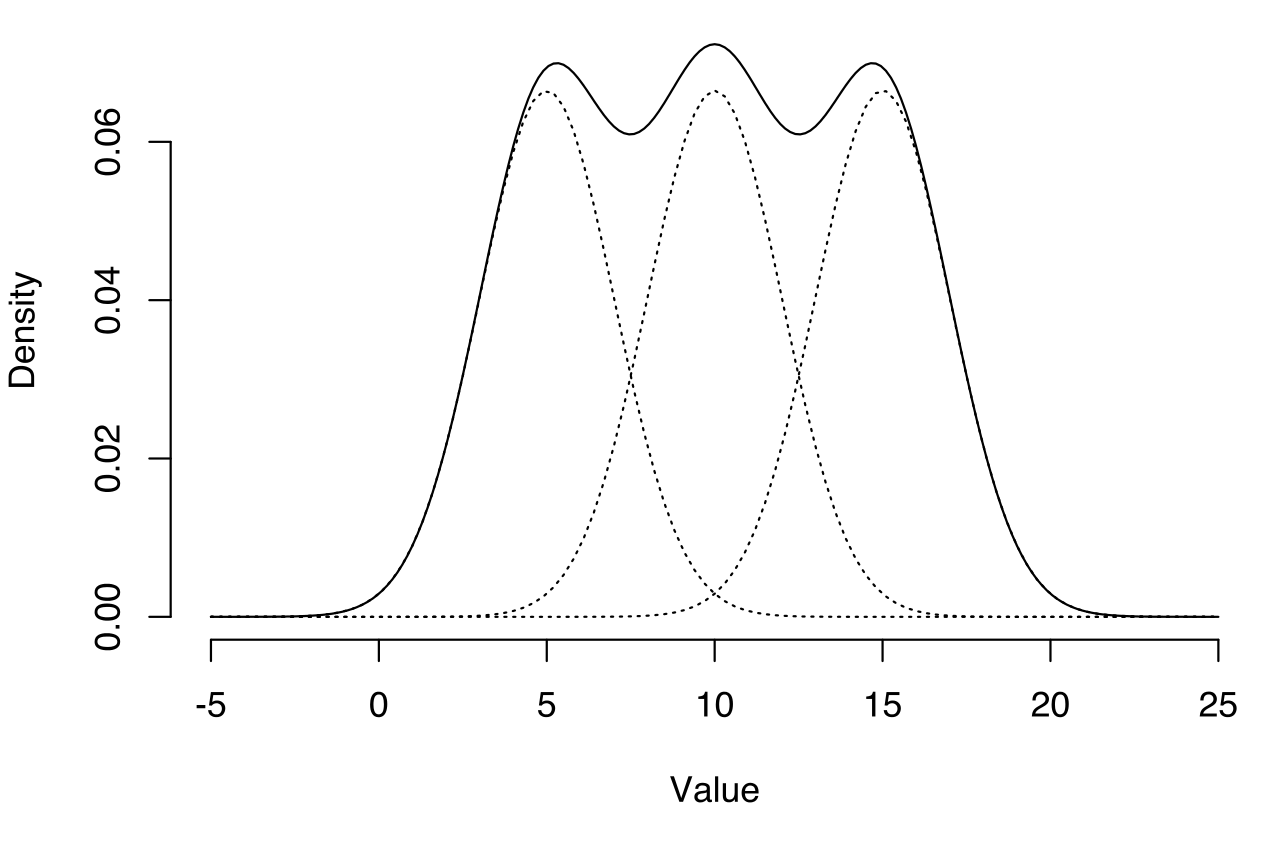
\includegraphics[width=0.6\textwidth]{fig/gaussian-mixture-distribution.png}
    \caption{混合分布}
    \label{fig:mix-dist}
\end{figure}

由于对数收益率的的可叠加性(较长时间内的对数收益率可分解为较短时间间隔对数收益率相叠加),并且利用上述正态分布性质,可知正态分布随机变量$d\ln S$(极短时间内)与叠加之后的$\Delta \ln S$(较长时间内)都应服从\textbf{正态分布}。

对比\textbf{比例收益率}在极短时间内(连续形式)与较长时间内(离散形式):
\begin{align*}
    \frac{dS_t}{S_t} &= \mu dt + \sigma dZ_t \\
    \frac{\Delta S_t}{S_t} &= \mu \Delta t + \sigma(Z_T - Z_t)
\end{align*}

百分比收益率虽然在极短时间(连续形式)服从正态分布。由于分母$S_t$不断改变,并不能通过叠加的形式得到较长时间的分布,即:
\begin{equation*}
    \frac{S_n - S_0}{S_0} \neq \frac{S_1- S_0}{S_0} + \frac{S_2-S_1}{S_1} + \dots + \frac{S_{n}-S_{n-1}}{S_{n-1}}
\end{equation*}

\textbf{存疑}:比例收益率在较短时间与较长时间应该也服从正态分布,通过累加两者服从的分布相同,变量不同,仅都服从同一正态分布。与对数收益率相比漂移项不同。且现实中比例收益率取值范围为$[-100\%,+\inf)$,并不符合正态分布,这点与模型不符。$\Delta S$则不服从正态分布,随着$S_t$的变化,其均值与方差也在不断改变。

\section{BSM 偏微分方程(PDE方法)}

\subsection{假设}
\begin{itemize}
    \item 人性假设
    \begin{itemize}[leftmargin=2em]
        \item 不存在无风险套利机会(无套利)
    \end{itemize}
    \item 完美世界
    \begin{itemize}
        \item 允许卖空标的证券
        \item 没有交易费用和税收
        \item 证券交易时连续的,价格变动也是连续的
        \item 所有证券都完全可分
    \end{itemize}
    \item 可交易资产
        \begin{itemize}
            \item 证券价格遵循几何布朗运动,即$\mu$和$\sigma$为常数
            \item 衍生品有效期内,无风险利率r为常数
            \item 衍生证券有效期内,标的证券没有现金收益支付
        \end{itemize}
\end{itemize}

\subsection{推导}

假设股票价格$S_t$遵循几何布朗运动,以及其离散形式有:
\begin{align*}
    d S_t & = \mu S_t dt + \sigma S_t d Z_t \\
    \Delta S_t & = \mu S_t \Delta t + \sigma S_t \Delta Z_t
\end{align*}

假设衍生品价格$f(S_t, t)$为$S_t$以及$t$的函数,根据伊藤引理可得其连续和离散形式有:

\begin{align*}
    df(S_t,t) & = \left(\frac{\partial f}{\partial S} \mu S_t  + \frac{\partial f}{\partial t} + \frac{1}{2}\frac{\partial^2 f}{\partial S^2} \sigma^2 S_t^2 \right)dt + \frac{\partial f}{\partial S} \sigma S_t dZ_t \\
    \Delta f(S_t,t) & = \left(\frac{\partial f}{\partial S} \mu S_t  + \frac{\partial f}{\partial t} + \frac{1}{2}\frac{\partial^2 f}{\partial S^2} \sigma^2 S_t^2 \right) \Delta t + \frac{\partial f}{\partial S} \sigma S_t \Delta Z_t
\end{align*}

由此可见,股票价格与衍生品价格的风险源均来自$\Delta Z_t$,因此可以构建投资组合,由一单位衍生品空头,以及$\partial f/\partial S$单位证券多头构成,进行对冲消除该风险源:
\begin{equation*}
    \Pi_t = -f_t + \frac{\partial f}{\partial S} S_t
\end{equation*}

在$\Delta t$时间内,该投资组合价值的变化$\Delta \Pi_t$来源其标的资产以及衍生品的价格变动,代入$\Delta S_t$与$\Delta f_t$可得:
\begin{align*}
    \Delta \Pi_t & = -\Delta f_t + \frac{\partial f}{\partial S} \Delta S_t \\
    & = -\left[ \left(\frac{\partial f}{\partial S} \mu S_t  + \frac{\partial f}{\partial t} + \frac{1}{2}\frac{\partial^2 f}{\partial S^2} \sigma^2 S_t^2 \right) \Delta t + \frac{\partial f}{\partial S} \sigma S_t \Delta Z_t \right] + \frac{\partial f}{\partial S} \left( \mu S_t \Delta t + \sigma S_t \Delta Z_t \right) \\
    & = -\left( \frac{\partial f}{\partial t} + \frac{1}{2}\frac{\partial^2 f}{\partial S^2} \sigma^2 S_t^2 \right) \Delta t
\end{align*}

由于此时组合消除了风险,因此组合只应获得无风险收益率:
\begin{align*}
    \Delta \Pi_t & = r \Pi_t \Delta t \\
    -\left( \frac{\partial f}{\partial t} + \frac{1}{2}\frac{\partial^2 f}{\partial S^2} \sigma^2 S_t^2 \right) \Delta t & =  r \left( -f_t + \frac{\partial f}{\partial S} S_t \right) \Delta t
\end{align*}

整理等式,消去$\Delta t$,即可得到\textbf{BSM偏微分方程}(Black-Scholes equation)。由于使用了Delta对冲的方法消除了其中的随机性,最终结果中并不包含任何随机过程,为普通的偏微分方程,为非随机微分方程。求解PDE需要给定的边界条件,如对于欧式看涨期权,其边界条件有当时间$t=T$到达其期限,期权价格$C=\max(S(T)-K,0)$。
\begin{equation*}
    \frac{\partial f}{\partial t} + r S_t \frac{\partial f}{\partial S} + \frac{1}{2} \sigma^2 S_t^2 \frac{\partial^2 f}{\partial S^2} = r f_t
\end{equation*}

\section{BSM公式(鞅方法)}

\subsection{风险中性世界}

\textbf{风险中性定价理论}就来源于BSM微分方程中的一个关键性质,在推导的过程中所有变量,如:股票价格、时间、波动率、无风险利率,均都不涉及投资者的风险偏好。在推导BSM微分方程中,使用Delta对冲方法消除了随机源之后。在不存在无风险套利的市场中,投资组合的收益率必须等于无风险收益率,否则就存在套利机会(\textbf{注意}:这一性质来源于无套利,而非假设)。因此最终结果中中并不包含预期收益率$\mu$,因为投资者对于风险的厌恶程度越高,其所要求的$\mu$也就越高。因此我们可以利用这个特点,即风险偏好在方程中不出现,即其可以随意取值,均不会影响方程的解。因此在计算期权价格中,可以使用任意风险偏好,而最简单的就是\textbf{假设所有投资者都是风险中性的}。所有投资的回报率期望均为无风险利率$r$,对风险中性的投资者而言,他们对风险的态度是中性的,因此不需要额外的风险溢酬。在一个风险中性世界里,任何现金流的现值都可以通过对其期望值以无风险利率贴现来得到。因此利用风险中性定价原理对衍生品定价的过程如下:
\begin{itemize}
    \item 假定标的资产的收益率期望为无风险利率(即假定$\mu=r$)
    \item 计算衍生产品到期时收益的期望
    \item 用无风险利率$r$对衍生品收益期望进行贴现。
\end{itemize}

风险中性定价是获得期权定价公式的一个人为工具或数学方法,其求得的解不但在风险中性世界中成立,在现实世界中也成立。当我们从风险中性世界换到风险厌恶世界时,两件事会发生:股票价格变动的增长率期望以及对衍生产品收益所必需使用的贴现率都将会变化,而这两种变化刚好相互抵消。

\subsection{BSM期权定价公式}

在风险中性世界中,看涨期权价值的期望为:
\begin{equation*}
    \rnE_t \left[ \max(S_T-K,0) \right]
\end{equation*}

欧式看涨期权的现值应为其在$T$时刻期望值以无风险利率进行贴现:
\begin{equation*}
    c = e^{-r(T-t)} \rnE_t \left[ \max(S_T-K,0) \right]
\end{equation*}

同时在风险中性世界下,漂移率$\mu$应等于无风险收益率r,因此有:
\begin{equation*}
    \ln S_T - \ln S_t \sim N \left((r-\frac{\sigma^2}{2})(T-t), \sigma^2(T-t)\right)
\end{equation*}

已知:
\begin{equation*}
    S_T = S_t \exp\left[\left(r-\frac{\sigma^2}{2}\right)\left(T-t\right) + \sigma\left(W_T - W_t \right)\right]
\end{equation*}

已知$Y = \frac{W_T - W_t}{\sqrt{T-t}} \sim N(0,1)$服从标准正态分布,其概率密度函数为:
\begin{equation*}
    \varphi(y) = \frac{1}{\sqrt{2\pi}} e^{-\frac{1}{2}y^2}
\end{equation*}

在风险中性下的期望,可以改写为如下积分的形式:
\begin{align*}
    \rnE_t \left[ \max(S_T-K,0) \right] & = \rnE_t \left[ S_t e^{(r-\frac{1}{2}\sigma^2)(T-t) + \sigma\sqrt{T-t}Y} - K \right]^+ \\
    & = \int_{-\infty}^{\infty} \left( S_t e^{(r-\frac{1}{2}\sigma^2)(T-t) + \sigma\sqrt{T-t}y} - K \right)^+ \varphi(y) dy
\end{align*}

当$S_t e^{(r-\frac{1}{2}\sigma^2)(T-t) + \sigma\sqrt{T-t}Y} - K \geq 0$时,有$y \geq \frac{ \ln (K/S_t) - (r-\frac{1}{2}\sigma^2)(T-t)}{\sigma\sqrt{T-t}}$,设其为$-d_2$,同时假设$d_1 = d_2 + \sigma \sqrt{T-t}$。
\begin{align*}
    \rnE_t \left[ \max(S_T-K,0) \right] & = \int_{-\infty}^{\infty} \left( S_t e^{(r-\frac{1}{2}\sigma^2)(T-t) + \sigma\sqrt{T-t}y} - K \right)^+ \varphi(y) dy \\
    & = S_t e^{(r-\frac{1}{2}\sigma^2)(T-t)} \int_{-d_2}^{\infty} e^{\sigma\sqrt{T-t} y} \varphi(y)dy - K\int_{-d_2}^{\infty} \varphi(y)dy \\
    & = S_t e^{(r-\frac{1}{2} \sigma^2) (T-t)} \int_{-d_2}^{\infty}{e^{\sigma\sqrt{T-t}y} \frac{1}{\sqrt{2\pi\ }}e^{-\frac{y^2}{2}}dy} - KN\left(d_2\right) \\
    & = S_t e^{r(T-t)} \int_{-d_2}^{\infty} \frac{1}{\sqrt{2\pi}} e^{\left( -\frac{\sigma^2 (T-t)}{2} + \sigma\sqrt{T-t}y - \frac{y^2}{2} \right)} dy - KN(d_2) \\
    & = S_t e^{r(T-t)} \int_{y = -d_2}^{y = \infty} \frac{1}{\sqrt{2\pi}}e^{-\frac{\left(y-\sigma\sqrt{T-t}\right)^2}{2}}dy - KN(d_2) \\
    &\hspace{4em} \text{(换元法:$u =y -\sigma\sqrt{T-t}$)} \\
    & =S_t e^{r(T-t)} \int_{u = -d_2-\sigma\sqrt{T-t}}^{u = \infty} \frac{1}{\sqrt{2\pi\ }}e^{-\frac{u^2}{2}}du - KN(d_2) \quad \text{($dy = du$)} \\
    & = S_t e^{r(T-t)} \int_{-d_1}^{\infty} \frac{1}{\sqrt{2\pi}}e^{-\frac{u^2}{2}} du - KN(d_2) \\
    & = S_t e^{r(T-t)}N(d_1) - KN(d_2)
\end{align*}

得到\textbf{BSM公式}(Black-Scholes formula),即欧式看涨期权的定价公式,其中$N(\cdot)$为标准正态分布的累积分布函数(CDF)。
\begin{equation*}
    \boxed{
        c = S_t N(d_1) - Ke^{-r(T-t)} N(d_2)
    }
\end{equation*}

并且已知期权平价公式:
\begin{equation*}
    c + K e^{r(T-t)} = p + S_t
\end{equation*}

将BSM看涨期权定价公式代入:
\begin{align*}
    p & = c + K e^{-r(T-t)} - S_t \\
    & = S_t N(d_1) - Ke^{-r(T-t)} N(d_2) +  Ke^{-r(T-t)} - S_t \\
    & = S_t (N(d_1) - 1) - K e^{-r(T-t)}(N(d_2)-1) \\
    & = S_t (-N(-d_1)) - K e^{-r(T-t)}(-N(-d_2)) \\
    & = K e^{-r(T-t)}N(-d_2) - S_t N(-d_1)
\end{align*}

可得欧式看跌期权定价公式,有:
\begin{equation*}
    \boxed{
    p = K e^{-r(T-t)}N(-d_2) - S_t N(-d_1)
    }
\end{equation*}

此时$d_1$和$d_2$分别为:
\begin{align*}
    d_1 &= \frac{\ln \frac{S_t}{K} + (r+\frac{1}{2}\sigma^2)(T-t)}{\sigma\sqrt{T-t}} \\
    d_2 &= \frac{\ln \frac{S_t}{K} + (r-\frac{1}{2}\sigma^2)(T-t)}{\sigma\sqrt{T-t}}
\end{align*}

\subsection{关于\texorpdfstring{$N(d_1)$}{TEXT}与\texorpdfstring{$N(d_2)$}{TEXT}}

对于期权,在定价时有两个不确定性需要考虑:
\begin{itemize}
    \item 期权到行权日到底是不是实值期权(In-The-Money),是否能够行权(能不能赚钱)
    \item 如果能行权了,那么收益的期望到底能有多少(能赚多少)
\end{itemize}

那么$N(d_1)$与$N(d_2)$对应了两个不确定性的概率,以欧式看涨期权为例。第二项比较容易理解,$N(d_2)$为在风险中性世界中,股票被行权的概率,即为$P(S_T>K)$。因此$Ke^{-r(T-t)}N(d_2)$为在当前时刻(折现后),考虑了行权概率后,所需支付的行权费成本。

第二项如果理解为成本,那么第一项代表着考虑行权概率后,当前时间点的股票收益期望。要能有收益,先决条件是能行权,即首先应有$S_T>K$。因此股票在行权时的价值应为一个条件期望$\E[S_T | S_T >K]$,是基于在行权价之上。此条件期望在乘以行权概率$N(d_2)$,并折现到当前时点,应为第一项。应有:
\begin{equation*}
    e^{r(T-t)} \E[S_T | S_T >K] N(d_2) = S_t N(d_1)
\end{equation*}

将上式中的$S_t$代换为$e^{r(T-t)}E[S_T]$:
\begin{equation*}
    e^{r(T-t)} \E[S_T | S_T >K] N(d_2) = S_t e^{r(T-t)}\E[S_T] N(d_1)
\end{equation*}

得到:
\begin{equation*}
    N(d_1) = \frac{\E[S_T | S_T >K]}{\E[S_T]} N(d_2)
\end{equation*}

由于最终的股票的收益并不独立于股票价格,这与行权价独立于股票价格不同,因此$N(d_1)$是基于股票价格加权后的行权概率。$N(d_1)$在数学上还有另外的解释,它是“以股票波动率$N(d_1)$为市场风险定价,并在以股票为计价单位时,期权被行权的概率”。

\subsection{使用BSM公式注意事项}

在实际使用过程,与进行计算的过程中有如下\text{注意点}
\begin{itemize}[leftmargin=4em]
    \item 在计算时,期限、漂移率(无风险利率)、波动率的时间单位应匹配(一般以年为单位,使用交易日计算)
    \item 由于只有交易日才有历史数据与收益率数据,波动率使用交易天数进行年化,中国240天左右,美国252天
    \item 无风险利率选择即期利率(Spot rate)而非到期收益率(YTM,真实收益率,票息5\%,但非平价发行)
    \item 波动率为一个时间窗口内(一般为年,252天交易日),日频连续复利收益率或对数收益率($\ln\frac{S_{t+1}}{S_{t}}$)标准差进行年化得到。
    \item 即日波动率乘以$\sqrt{252}$(一天的方差为$s^2$,由于方差可加,252个交易日的方差即为$s^2 \times 252$,标准差或波动率为$s\sqrt{252}$)。同理,月频收益率得到的波动率应乘以$\sqrt{252/21}$进行年化。
    \item 如果到期时间(time to maturity)是根据日历日(calendar day)计算,那么此时的隐含波动率则为每日历日(per calendar day),而VIX计算是根据交易日(trading day),因此进行转换,并根据计算的日历日或交易日进行年化。
\end{itemize}

\section{希腊值}

BSM定价公式的核心价值在于它构建了量化数学模型,以此可以计算期权的各种风险敞口,这对于将期权交易者至关重要。由BSM公式出发可以方便的求出期权价格对标的资产、时间、利率、波动率的偏导数,从而确定期权在这些因素上的风险敞口,常见的风险敞口由五类,由希腊字母表示,称为\text{希腊值},分别是:Delta、Gamma、Vega、Theta与Rho。

\subsection{正态分布与性质}

对于正态分布或高斯分布(Gaussian distribution),其\textbf{概率密度函数}(Probability Density Function,PDF):
\begin{equation*}
    f(x;\mu,\sigma) = \frac{1}{\sigma\sqrt{2\pi}} e^{-\frac{1}{2}\left(\frac{x-\mu}{\sigma} \right)^2}
\end{equation*}

则有$N(x)$为标准正态分布(Standard normal distribution)的\textbf{累积分布函数}(CDF,Cumulative Distribution Function)为:
\begin{equation*}
    N(x) = \frac{1}{\sqrt{2\pi}} \int_{-\infty}^{x}e^{-\frac{z^2}{2}}dz
\end{equation*}

则有$N'(x)$为标准正态分布的概率密度函数:
\begin{equation*}
    N'(x) = \frac{1}{\sqrt{2\pi}} e^{-\frac{x^2}{2}}
\end{equation*}

由于正态分布的对称性,易知有如下性质:
\begin{equation*}
    N(-x) = 1-N(x) \qquad \qquad
    N'(x) = N'(-x)
\end{equation*}

\subsection{希腊值定义}

定义衍生品价格,对标的价格的一阶导为Delta,对标的价格的二阶导为Gamma,对于期限的一阶导为Theta,对于无风险利率的一阶导为Rho,对于波动率的一阶导为Sigma。
\begin{equation*}
    \text{Delta} = \frac{\partial V}{\partial S} \quad 
    \text{Gamma}  = \frac{\partial^2 V}{\partial S^2} \quad
    \text{Theta} = -\frac{\partial V}{\partial \tau} \quad
    \text{Rho} = \frac{\partial V}{\partial r} \quad
    \text{Vega} = \frac{\partial V}{\partial\sigma} \quad
\end{equation*}

\subsection{Black模型}

\begin{align*}
    C &= e^{-r\tau}[FN(d_1) - KN(d_2)] \\
    P &= e^{-r\tau}[KN(-d_2) - FN(-d_1)]
\end{align*}

其中有:
\begin{align*}
    d_1 &= \frac{\ln(F/K) + \sigma^2/2\tau}{\sigma \sqrt{\tau}} \\
    d_2 &= \frac{\ln(F/K) + \sigma^2/2\tau}{\sigma \sqrt{\tau}} \\
    d_2 &= d_1 - \sigma \sqrt{\tau}
\end{align*}

\begin{equation*}
    \frac{\partial d_1}{\partial F} = \frac{\partial d_2}{\partial F} = \frac{\frac{\partial \ln(F/K)}{\partial F} \sigma \sqrt{\tau}}{(\sigma \sqrt{\tau})^2} = \frac{\partial (\ln F - \ln K)/\partial F}{\sigma\sqrt{\tau}} = \frac{1}{F\sigma\sqrt{\tau}}
\end{equation*}

\subsubsection{Delta}

\begin{align*}
    FN'(d_1) &= \frac{F}{\sqrt{2\pi}}e^{-d_1^2/2} \\
    KN'(d_2) &= \frac{K}{\sqrt{2\pi}}e^{-d_2^2/2} = \frac{K}{\sqrt{2\pi}}e^{-d_1^2/2+d_1\sigma\sqrt{\tau}-\sigma^2\tau/2} \\
    &= \frac{K}{\sqrt{2\pi}}e^{-d_1^2/2+\ln(F/K)} 
    \qquad \left(d_1\sigma\sqrt{\tau} = \ln(F/K)+\sigma^2\tau\right) \\
    &= \frac{F}{\sqrt{2\pi}}e^{-d_1^2/2} \\
    &= FN'(d_1) \\
    \text{Delta}_C &= e^{-r\tau}[N(d_1) + FN'(d_1)\frac{\partial d_1}{\partial F} - KN'(d_2)\frac{\partial d_2}{\partial F}] \\
    &= e^{-r\tau}N(d_1) \\
    \text{Delta}_P &= e^{-r\tau}[KN'(-d_2)\frac{\partial d_2}{\partial F} - N(-d_1) - FN'(-d_1)\frac{\partial d_1}{\partial F}] \\
    &= e^{-r\tau}(-N(-d_1)) \qquad \left(KN'(-d_2) = KN'(d_2),\, FN'(-d_1)= FN'(d_1)\right) \\
    &= e^{-r\tau}(N(d_1)-1)
\end{align*}

\subsection{BSM模型}

当红利率为$q$时,有:
\begin{align*}
    C_t &= S_te^{-q\tau}N(d_1) - Ke^{-r\tau}N(d_2) \\
    P_t &= -S_te^{-q\tau}N(-d_1) + Ke^{-r\tau}N(-d_2)
\end{align*}

其中有:
\begin{align*}
    d_1 &= \frac{\ln(S/K) + (r+-q+\frac{\sigma^2}{2})\tau}{\sigma \sqrt{\tau}} \\
    d_2 &= \frac{\ln(S/K) + (r-q-\frac{\sigma^2}{2})\tau}{\sigma \sqrt{\tau}} \\
    d_2 &= d_1 - \sigma \sqrt{\tau}
\end{align*}

\begin{lemm}
    \begin{equation*}
        \frac{\partial d_2}{\partial S} = \frac{\partial d_1}{\partial S} = \frac{\frac{\partial \ln(S/K)}{\partial S} \sigma \sqrt{\tau}}{(\sigma \sqrt{\tau})^2} = \frac{\partial (\ln S - \ln K)/\partial S}{\sigma\sqrt{\tau}} = \frac{1}{S\sigma\sqrt{\tau}}
    \end{equation*}
    \begin{equation*}
        \frac{\partial d_2}{\partial \tau} = \frac{\partial d_1}{\partial \tau} - \frac{1}{2}\frac{\sigma}{\sqrt{\tau}}
    \end{equation*}
    \begin{equation*}
        \frac{\partial d_2}{\partial \sigma} = \frac{\partial d_1}{\partial \tau} - \sqrt{\tau}
    \end{equation*}
    \begin{equation*}
        \frac{\partial d_2}{\partial r} = \frac{\partial d_1}{\partial r}
    \end{equation*}
\end{lemm}

\begin{lemm}
    对于BSM公式,有:
    \begin{equation*}
        S_t N'(d_1) = Ke^{-r\tau} N'(d_2)
    \end{equation*}
\end{lemm}

\begin{proof}
    已知:
    \begin{align*}
        d_2^2-d_1^2 &= (d_2-d_1)(d_2+d_1) \\
        &= (-\sigma\sqrt{\tau})(2d_1-\sigma\sqrt{\tau}) \\
        &= (-\sigma\sqrt{\tau})\left(\frac{2\ln(S_t/K) + 2(r+\sigma^2/2)\tau}{\sigma\sqrt{\tau}} -\sigma\sqrt{\tau}\right) \\
        &= -2\left[\ln\frac{S_t}{K}+r\tau\right]
    \end{align*}

    同时已知$N'(x)=\frac{1}{\sqrt{2\pi}} e^{-\frac{x^2}{2}}$,则有:
    \begin{equation*}
        \ln\left(\frac{N'(d_1)}{N'(d_2)}\right)
        = -\frac{d_1^2}{2} + \frac{d_2^2}{2}
        = \frac{1}{2} (d_2^2-d_1^2)
        = -\left[\ln\frac{S_t}{K} +r\tau\right]
    \end{equation*}

    对等式两边取指数:
    \begin{align*}
        \frac{N'(d_1)}{N'(d_2)} 
        &= \exp\left( -\left[\ln\frac{S_t}{K} +r\tau\right] \right) \\
        &= \exp \left( \ln\frac{K}{S_t}-r\tau \right) \\
        &= \frac{K}{S_t} e^{-r\tau} \\
        S_t N'(d_1) &= Ke^{-r\tau} N'(d_2)
    \end{align*}
\end{proof}

\subsubsection{Delta}

对于无红利,即$q=0$时,Delta($\Delta$)有:
\begin{align*}
    \text{Delta}_C &= \frac{\partial C}{\partial S}
    = N(d_1) + \frac{1}{S_t\sigma\sqrt{\tau}} \left[ S_t N'(d_1)-Ke^{-r\tau}N'(d_2) \right] = N(d_1) \\
    \text{Delta}_P &= \frac{\partial P}{\partial S}
    = -N(-d_1) + \frac{1}{S_t\sigma\sqrt{\tau}} \left[ S_t N'(d_1)-Ke^{-r\tau}N'(d_2) \right] = N(d_1)-1
\end{align*}

当已知红利率时,有:
\begin{align*}
    \text{Delta}_C &= -e^{-q\tau} N(d_1) \\
    \text{Delta}_P &= -e^{-q\tau} N(-d_1)
\end{align*}

\subsubsection{Gamma}

对于Gamma($\Gamma$)而言,看涨与看跌期权Gamma相同:
\begin{equation*}
    \text{Gamma} = \frac{\partial^2 V}{\partial S^2} = \frac{\partial N(d_1)}{\partial S} = N'(d_1)\frac{\partial d_1}{\partial S} = \frac{N'(d_1)}{S\sigma\sqrt{\tau}}
\end{equation*}

\subsubsection{Vega}

对于Vega而言,看涨与看跌期权Vega相同
\begin{equation*}
    \text{Vega} = \frac{\partial V}{\partial \sigma}  = SN'(d_1)\sqrt{\tau}
\end{equation*}

当红利率为$q$时有:
\begin{equation*}
    \text{Vega}_C = \text{Vega}_P = S e^{-q\tau}N'(d_1)\sqrt{\tau}
\end{equation*}

推导:
\begin{align*}
    \text{Vega} &= \frac{\partial C}{\partial \sigma} = \frac{\partial}{\partial \sigma} \left[S N(d_1) - K e^{-r\tau}N(d_2)\right] \\
    &= S N'(d_1) \frac{\partial d_1}{\partial \sigma} - Ke^{-r\tau}N'(d_2) \frac{\partial d_2}{\partial \sigma} \\
    &= S N'(d_1) \frac{\partial d_1}{\partial \sigma} - Ke^{-r\tau}N'(d_2) \left[ \frac{\partial d_1}{\partial \sigma} -\sqrt{\tau} \right] \qquad \text{(对$d_2 = d_1 - \sigma\sqrt{\tau}$求导)} \\
    &= \left[ S N'(d_1) - Ke^{-r\tau}N'(d_2) \right] \frac{\partial d_1}{\partial \sigma} + Ke^{-r\tau}N'(d_2) \sqrt{\tau} \\
    &= S N'(d_1)\sqrt{\tau} \qquad \text{(已知$S N'(d_1) = Ke^{-r\tau}N'(d_2)$)}
\end{align*}

\subsubsection{Theta}

对于欧式看涨期权有其Theta($\Theta$):
\begin{equation*}
    \text{Theta}_C = \frac{\partial C}{\partial \tau} = -\frac{S_t N'(d_1)\sigma}{2\sqrt{\tau}} - r K e^{-r\tau}N(d_2)
\end{equation*}

证明:
\begin{align*}
    \text{Theta}_C &= -\frac{\partial C}{\partial \tau} = - \frac{\partial [S_t N(d_1) - Ke^{-r\tau} N(d_2)]}{\partial \tau} \\ 
    &= -\frac{\partial S_t N(d_1)}{\tau} + \frac{\partial Ke^{-r\tau} N(d_2)}{\partial \tau} \\ 
    &= -S_t N'(d_1)\frac{\partial d_1}{\partial \tau} - rKe^{-r\tau}N(d_2) + Ke^{-r\tau} N'(d_2)\frac{\partial d_2}{\partial \tau} \\
    &= -S_t N'(d_1)\frac{\partial d_1}{\partial \tau} - rKe^{-r\tau} N(d_2) + Ke^{-r\tau}N'(d_2)\left(\frac{\partial d_1}{\partial \tau} -\frac{1}{2}\frac{\sigma}{\sqrt{\tau}} \right) \\
    &= \frac{\partial d_1}{\partial \tau} \left[\cancel{-S_t N'(d_1) + Ke^{-r\tau} N'(d_2) } \right] + Ke^{-r\tau} \left[ -rN(d_2) -\frac{1}{2}\frac{\sigma}{\sqrt{\tau}} N'(d_2)\right] \\
    &=  -\frac{1}{2}\frac{\sigma}{\sqrt{\tau}}S_t N'(d_1) - rKe^{-r\tau} N(d_2)
\end{align*}

对于欧式看跌期权有:
\begin{equation*}
    \text{Theta}_P = \frac{\partial P}{\partial \tau} = -\frac{S_t N'(d_1)\sigma}{2\sqrt{\tau}} + r K e^{-r\tau}N(-d_2)
\end{equation*}

证明:
\begin{align*}
    \text{Theta}_P &= -\frac{\partial P}{\partial \tau} = - \frac{\partial [-S_t N(-d_1) + Ke^{-r\tau} N(-d_2)]}{\partial \tau} \\ 
    &= \frac{\partial S_t N(-d_1)}{\tau} - \frac{\partial Ke^{-r\tau} N(-d_2)}{\partial \tau} \\ 
    &= S_t N'(-d_1)\frac{\partial d_1}{\partial \tau} + rKe^{-r\tau}N(-d_2) - Ke^{-r\tau} N'(-d_2)\frac{\partial d_2}{\partial \tau} \\
    &= S_t N'(d_1)\frac{\partial d_1}{\partial \tau} + r Ke^{-r\tau} N(-d_2) - Ke^{-r\tau}N'(d_2)\left(\frac{\partial d_1}{\partial \tau} -\frac{1}{2}\frac{\sigma}{\sqrt{\tau}} \right) \\
    &= \frac{\partial d_1}{\partial \tau} \left[\cancel{S_t N'(d_1) - Ke^{-r\tau} N'(d_2) } \right] + Ke^{-r\tau} \left[ rN(-d_2) -\frac{1}{2}\frac{\sigma}{\sqrt{\tau}} N'(d_2)\right] \\
    &=  -\frac{1}{2}\frac{\sigma}{\sqrt{\tau}}S_t N'(d_1) + rKe^{-r\tau} N(-d_2) \\
    &=  -\frac{1}{2}\frac{\sigma}{\sqrt{\tau}}S_t N'(d_1) + rKe^{-r\tau}[1- N(d_2) ] = \text{Theta}_c + rKe^{-r\tau}
\end{align*}

另有,利用Put-Call Parity可知:
\begin{equation*}
    C + Ke^{-r\tau} = P + S_t \qquad \Rightarrow \qquad \frac{\partial C}{\partial \tau} - rKe^{-r\tau} = \frac{\partial P}{\partial \tau} 
\end{equation*}

等式两边对$\tau$求偏导:
\begin{align*}
    -\frac{\partial P}{\partial \tau} & = -\frac{\partial C}{\partial \tau} + rKe^{-r\tau} \\
    \text{Theta}_P &= \text{Theta}_C + rKe^{-r\tau}
\end{align*}

\subsubsection{Rho}

欧式看涨期权,对无风险利率求导可得:
\begin{align*}
    \text{Rho}_C &= \frac{\partial C}{\partial r} = 
    \frac{\partial [S_t N(d_1) - Ke^{-r\tau} N(d_2)]}{\partial r} \\
    &= S_t N'(d_1) \frac{\partial d_1}{\partial r} - Ke^{-r\tau} N'(d_2)\frac{\partial d_2}{\partial r} + \tau K e^{-r\tau} N(d_2) \\
    &= \frac{\partial d_1}{\partial \tau} \left[\cancel{S_t N'(d_1) - Ke^{-r\tau} N'(d_2) } \right] + \tau K e^{-r\tau} N(d_2) \\
    &= \tau K e^{-r\tau} N(d_2)
\end{align*}

同理,对于欧式看跌期权:
\begin{align*}
    \text{Rho}_P &= \frac{\partial P}{\partial r} = 
    \frac{\partial [-S_t N(-d_1) + Ke^{-r\tau} N(-d_2)]}{\partial r} \\
    &= -S_t N'(d_1) \frac{\partial d_1}{\partial r} + Ke^{-r\tau} N'(-d_2)\frac{\partial d_2}{\partial r} - \tau Ke^{-r\tau} N(-d_2) \\
    &= \frac{\partial d_1}{\partial \tau} \left[\cancel{-S_t N'(d_1) + Ke^{-r\tau} N'(d_2) } \right] - \tau K e^{-r\tau} N(-d_2) \\
    &= -\tau K e^{-r\tau} N(-d_2)
\end{align*}

\subsection{Delta对冲}
Delta为衍生品价格变动与其标的资产价格变动的比率。如果假定股票价格(X)与期权价格(Y)为折线,则其斜率应为Delta,即对股票价格变动一单位,期权价格变动$\Delta$单位。而现实中并非折线,Delta则为两者切线斜率。
\begin{equation*}
    \Delta = \frac{\partial V}{\partial S}
\end{equation*}

而从持有标的资产和衍生品数量分别为$N_S$和$N_V$而言,为了维持对冲结果,易知对于每一单位标的资产,应使用$\Delta$单位衍生品进行对冲。
\begin{equation*}
    \Delta V \times N_V = \Delta S \times N_S \qquad \Rightarrow \qquad
    \Delta = \frac{\partial V}{\partial S} = \frac{N_S}{N_V}
\end{equation*}

而对于投资组合而言,其净Delta(Net portfolio delta)应为组合内所有某合约Delta与该合约数量乘积之和:
\begin{equation*}
    \sum_{i=1}^{n} \text{Delta}_i \times \text{期权合约数}_i
\end{equation*}

同样对于Vega而言,投资组合净Vega(Net portfolio vega)为:
\begin{equation*}
    \sum_{i=1}^{n} \text{Vega}_i \times \text{期权合约数}_i
\end{equation*}

假定股票价格遵循几何布朗运动,则有在现实测度(Physical probability measure)下:
\begin{equation*}
    \frac{dS_t}{S_t} = \mu dt + \sigma dW_t
\end{equation*}

根据伊藤引理:
\begin{equation*}
    f(T,W_T) =f(t,W_t) = \int^T_t \frac{\partial f}{\partial u}du + \int^T_t \frac{\partial f}{\partial S} dW_t \frac{1}{2} + \int^T_t\frac{\partial ^2 f}{\partial S^2} 
\end{equation*}

【待整理】 在Bakshi and Kapadia 2003中,

在一段时间内的使用看涨看跌期权进行Delta对冲(\textbf{注意:}由几何布朗运动与伊藤过程推到而来,因此看涨看跌期权形式相同,买入看涨看跌期权,并卖出股票,净投资金额获得无风险收益)。
\begin{equation*}
    \text{Call Gain} = C_{t+\tau} - C_t - \Delta_t ( S_{t+\tau}-S_t) - \frac{r\tau}{365}(C_{t+\tau} - \Delta_t S_t)
\end{equation*}
\begin{equation*}
    \text{Put Gain} = P_{t+\tau} - P_t - \Delta_t ( S_{t+\tau}-S_t) - \frac{r\tau}{365}(P_{t+\tau} - \Delta_t S_t)
\end{equation*}

Long call, short delta stock/ short call, long delta stock

Long put, long delta stock/ short put, short delta stock

\subsection{泰勒级数}

级数为无穷的序列(sequences)(或无穷多项)的和。泰勒级数(Taylor series)使用无限项序列来表示一个函数,每项由该函数在某一点的导数求得。一个函数的有限项的泰勒级数叫做泰勒多项式(Taylor polynomial)。对于一元函数在$x=a$处展开的泰勒级数有:
\begin{align*}
    f(x) &= \sum^{\infty}_{n=0} \frac{f^{(n)}(a)}{n!}(x-a)^n \\
    &= \frac{f(a)}{1}(1)+ \frac{f'(a)}{1}(x-a) + \frac{f''(a)}{2}(x-a)^2 + \frac{f'''(a)}{6}(x-a)^3 + \dots \\
    &= f(a) + f'(a)(x-a) + \frac{f''(a)}{2}(x-a) + \frac{f'''(a)}{6}(x-a)^3 + \dots
\end{align*}

对于多元函数在$(a,b)$处展开的泰勒级数为:
\begin{align*}
    f(x,y) &= f(a,b) + f'_x(a,b)(x-a) + f'_y(a,b)(y-b) \\
    &\quad + \frac{1}{2}f''_{xx}(a,b)(x-a)^2 + \frac{1}{2}f''_{yy}(a,b)(y-b)^2 +\cancel{2*\frac{1}{2}}f''_{xy}(a,b)(x-a)(y-b)
\end{align*}

\subsubsection*{原理}
假设使用多项式$P(x) = c_0 + c_1 (x-a) + c_2 (x-a)^2 + \dots$近似原函数。则应有多项式与原函数,从零阶导开始至$n$阶导,在$x=a$点的取值都与原函数相同(即从单个点,提取原函数所有导数信息):
\begin{itemize}
    \item $x-a$使得带入a进行计算时,除了当前导数对应次数的项之外都等于零。如原函数在$a$点的二阶导$f''(a)$,对应泰勒级数$x$二次项的系数$c_2$:一阶导为$P'(x) = c_1 + 2c_2(x-a)+\dots$,二阶导为$P''(x) = 2c_2 + 3c_3(x-a)^2 + \dots$,则有$P''(a) = 2c_2 = f''(a)$,此时$c_2 = \tfrac{f''(a)}{2}$
    \item 小于当前求导次数的泰勒级数项,由于求导都为零(如上所示求二阶导后,常数项与一次项都为0),使得多项式每一项的系数$c_n$都独立对应原函数n阶导数值
    \item 系数为$\frac{1}{n!}$是为了取消多次求导的影响,如$P'''(x)=3 \cdot 2 \cdot 1 \cdot c_3(x-a) + \cdots$
\end{itemize}

\subsection{对冲参数}

假设投资组合$\Pi$为标的资产价格$S$与时间$t$的函数,则有在$(S_0,t_0)$展开为:
\begin{align*}
    \Pi(S,T) &= \Pi(S_0,t_0) + \frac{\partial \Pi}{\partial S}(S-S_0) + \frac{\partial \Pi}{\partial t}(t-t_0) \\
    &\quad + \frac{1}{2}\frac{\partial^2 \Pi}{\partial S^2}(S-S_0)^2 + \frac{1}{2}\frac{\partial^2 \Pi}{\partial t^2}(t-t_0)^2 + \frac{\partial^2 \Pi}{\partial S \partial t}(S-S_0)(t-t_0) + \dots
\end{align*}

整理可得:
\begin{equation*}
    \Delta \Pi = \frac{\partial \Pi}{\partial S}\Delta S + \frac{\partial \Pi}{\partial t}\Delta t + \frac{1}{2}\frac{\partial^2 \Pi}{\partial S^2}\Delta S^2 + \frac{1}{2}\frac{\partial^2 \Pi}{\partial t^2}\Delta t^2 + \frac{\partial^2 \Pi}{\partial S \partial t}\Delta S \Delta t + \dots
\end{equation*}

将阶数高于$\Delta t$的项忽略(前三项之后),可以发现对于一个Delta中立的投资组合,应有\footnote{见OFOD第十版附录19A\label{ofod_19a}}:
\begin{equation*}
    \Delta \Pi = \Theta \Delta t + \frac{1}{2} \Gamma \Delta S^2
\end{equation*}

在实践中,波动率并非为常数。在短时间内忽略无风险利率的变化,仅仅关注标的资产价格$S$以及隐含波动率$\sigma_{imp}$作为期权价格$V$的近似,则有\footref{ofod_19a}:
\begin{equation*}
    \Delta V = \frac{\partial V}{\partial S}\Delta S + \frac{\partial V}{\partial \sigma_{imp}}\Delta \sigma_{imp} + \frac{1}{2} \frac{\partial^2 V}{\partial S^2}\Delta S^2 + \frac{1}{2} \frac{\partial^2 V}{\partial \sigma^2_{imp}} \Delta \sigma^2_{imp} + \frac{\partial^2 V}{\partial S \partial \sigma_{imp}}\Delta S \Delta \sigma_{imp} + \dots
\end{equation*}

可见delta、vega、gamma对应了上式中的前三项。而交易员也将$\tfrac{\partial^2 V}{\partial \sigma^2_{imp}}$称为Vomma,即Vega对于$\sigma_{imp}$的敏感程度,或Vega的Vega。将$\tfrac{\partial^2 V}{\partial S\partial \sigma_{imp}}$称为Vanna,或理解为Delta的Vega,即对于$\sigma_{imp}$的变动,Delta的敏感程度。

\section{波动率}

波动率为一种风险的度量,所有的计算方法都是一种近似估计,并不代表准确的波动率。波动率可以大致分为两类,一类为回望波动率(backward looking),一类为前瞻波动率(forward looking)。两者的区别在于回望波动率使用的是一段时间内的历史数据所计算出来的,是已经发生的波动率,如:历史波动率、已实现波动率、GARCH波动率。而前瞻法或隐含法,是未来一段时间内波动率的期望,由于在期权交易中,所有的交易者都必须估计未来波动率,并以此为基础进行交易。因此在一个充分竞争的环境中,最后期权价格中的隐藏波动率就包含了市场对未来波动率的预期。具体而言可分为有模型法(如BS隐含波动率)和无模型法(为风险中性预期:风险中性预期=现实预期-波动率风险溢酬=现实理性预期+投资者情绪-波动率风险溢酬)。

波动率的数学定义为:假设$r_t$为一个资产的收益率时间序列,有$t=1,2,3,\dots,T$,则有样本方差为:
\begin{equation*}
    \sigma^2(r_t) = \frac{1}{T-1} \sum^T_{t=1} (r_t - \bar{r})^2 
\end{equation*}

其中样本均值应有:
\begin{equation*}
    \bar{r} = \frac{1}{T} \sum_{t=1}^{T}r_t
\end{equation*}

\subsection{历史波动率}

历史波动率(Historical volatility)是基于历史信息得到的,指资产收益率在过去一段时间内表现出的波动水平,可以由资产收益率在过去一段时间内的标准差计算得到。一般使用日频数据,如计算:过去30个交易日的标准差。

【待核实】在 Black Scholes 的框架下,也就是假设股票价格服从 GBM 的时候,historical volatility 可以用 quadratic variation 计算。如下式:
\begin{equation*}
    \lim_{n\rightarrow \infty} \sum^{n}_{i=1}(X_{t_i} - X_{t_{i-1}})^2 = [X,X]_T = \sigma^2 T
\end{equation*}

其中$X_t$为股票价格的对数,$t_0,t_1,\dots,t_n$为$[0,T]$区间的一个划分。注意,这个和标准差不一样,这个其实是对数收益率的二阶距。可以证明,用 quadratic variation 得到的估计量是一致估计。???

BSIV与MFIV为风险中性下的波动率


\subsection{已实现波动率}

【待整理】已实现波动率(Realized volatility),顾名思义,为已发生的波动率。

一种为特定针对隐含波动率,目的用于对比,对应的已实现波动率。即如在t-30天的时点,观察未来30天的隐含波动率,而后在t时间,观察已发生的30日之内的历史波动率。

一种为针对频率较高的数据计算的一种波动率,又称为日内波动率或高频波动率。高频数据是指以小时、分钟或秒为采集频率的数据。一般使用日内高频频率为5分钟。为:
\begin{equation*}
    \text{RV}_t = \sum^{T}_{i=1} r^2_{t} = \sum^{N}_{i=1} \left( \ln \frac{S_{t}}{S_{t-1}} \right)^2
\end{equation*}

以上只是最基础的计算日内高频波动率的方法,还有其他的计算日内波动率的方式如:
\begin{itemize}
    \item Garman和Klass(1980)
    \item Andersen和Bollerslev(1998)
    \item Hansen和Lunde(2005)
    \item ...
\end{itemize}

\subsection{GARCH波动率}

GARCH为广义自回归条件异方差模型(Generalized autoregressive conditional heteroskedasticity)。Robert Engle于1982年在《计量经济学》上提出了ARCH模型用于估计和预测波动率。在此基础上,Bollerslev(1986)建立了广义自回归条件异方差(GARCH)模型。

【核实】
EWMA方法即指数移动平均方法。EWMA根据历史数据距当前时刻的远近,分别赋予不同的权重,距离现在越近,赋予的权重越大,我们认为越远的历史信息所起的作用越小,因此计算波动率时所赋予的权重越小。GARCH与EWMA都使用到了指数移动平均,他们都赋予最近的信息以更大的权重,EWMA事实上是一种特殊形式的GARCH。

GARCH(1,1)模型方差如下:
\begin{equation*}
    \sigma^{2}_{t} = a + b r^{2}_{t-1,t} + c \sigma^{2}_{t-1}
\end{equation*}

当取$a=0$,$b+c=1$时,上式子有:
\begin{equation*}
    \text{GARCH}(1,1) = a + b r^{2}_{t-1,t} + (1-b) \sigma^{2}_{t-1}
\end{equation*}

同时又EWAM为
\begin{equation*}
    \text{EWMA} = a + \lambda r^{2}_{t-1,t} + (1-\lambda) \sigma^{2}_{t-1}
\end{equation*}

\subsubsection{GJR-GARCH波动率}

\begin{gather*}
    \sigma^2_t = \omega + \left( \alpha + \gamma I_{t-1]} \right) \varepsilon_{t-1}^2 + \beta \sigma_{t-1}^2 \\
    r_t = \mu + \varepsilon_t \\
    \varepsilon_t = \sigma_t z_t
\end{gather*}

\begin{equation*}
    I_{t-1} = 
    \begin{cases}
        0 \quad\text{if}\quad r_{t-1} \geq \mu \\
        1 \quad\text{if}\quad r_{t-1} < \mu 
    \end{cases}
\end{equation*}

\subsection{随机波动率}

随机波动率(Sochastic volatility)指随机过程的波动率为随机变量。
% https://en.wikipedia.org/wiki/Stochastic_volatility
\begin{itemize}
    \item Heston model
    \item SABR
    \item CEV(Constant elasticity of variance model)
    \item Local volatility
\end{itemize}

\subsubsection{局部波动率}

【核实】Local volatility,这个其实是一个作为 stochastic volatility 的一种替代做法,就是认为 volatility 是一个关于时间和资产价格的确定性函数$\sigma(t,S_t)$ ,因此也叫 Deterministic Volatility Function (DVF)。这样做也就是为了避免 Heston Model 等 stochastic volatility 带来的计算复杂度。Dupire 给出了一种计算 local volatility 的方法:
\begin{equation*}
    \sigma^2(K,T) = \frac{\frac{\partial C}{\partial T}}{\frac{1}{2} K^2 \frac{\partial^2 C}{\partial K^2}}
\end{equation*}

\subsection{隐含波动率}

如上文所述,隐含波动率(Implied volatility)指并不使用历史数据进行预测,从市场价格中得到的波动率信息。因为在一个充分竞争的市场交易之中,市场当前的价格已经包含了对未来波动率的预期,因此只需要将波动率信息从当前市场价格信息中提取出来。因为波动率隐藏在市场价格之中,称之为隐含波动率。

【待核实】由于是根据期权市场价格求得,实际为风险中性下的,标的证券在到期日之内波动率的期望。而实际中,证券存续的时间远远超过期权存续的时间。因此隐含波动率,与现实波动率存在两个方向的差异,第一是风险中性测度与现实测度的差异,即不考虑风险溢酬,第二为存续时间的差异,期权存续时间较短,而股票存续时间较长,在较长的时间内波动应该相对更为平稳。

\subsubsection{BS隐含波动率}

假定市场上的期权或者权证的交易价格满足Black-Scholes-Merton(BSM)期权定价公式,将市场上可以观测到的标的资产价格($S$)、执行价格($K$)、利率($r$)、期限($\tau$)作为已知变量代入定价公式中,则可以得到期权当前的市场价格所隐含的波动率,此时提取的为期限内的波动率(option-implied volatility expectations until expiration),BS隐含波动率(BS implied volatility)为未来波动率的预期。
\begin{align*}
    c &= S_t N(d_1) - Ke^{-r(T-t)} N(d_2) \\
    p & = K e^{-r(T-t)}N(-d_2) - S_t N(-d_1) \\
    d_1 &= \frac{\ln \frac{S_t}{K} + (r+\frac{1}{2}\sigma^2)(T-t)}{\sigma\sqrt{T-t}} \\
    d_2 &= \frac{\ln \frac{S_t}{K} + (r-\frac{1}{2}\sigma^2)(T-t)}{\sigma\sqrt{T-t}} = d_1 - \sigma\sqrt{T-t}
\end{align*}

\subsubsection{无模型波动率}

虽然一般将无模型波动率(Model-free implied volatility)认为是“BS隐含波动率的一种加权平均”更方便理解,但事实上无模型波动率与BS模型完全没有关系。虽然早期的VIX是由8个期权的隐含BS波动率加权得到的30天(日历日或22天交易日)波动率预期(Whaley 1993),但现今已更新为无模型波动率。且发布时是根据S\&P100(OEX),因为其交易量较大,而当时S\&P500(SPX)交易量只有其五分之一。

如计算BS隐含波动率,使用这样的方法估计未来波动率的预期,其本质是基于BS期权定价模型的,即根据定价模型去拟合市场的价格,从而得到其中隐含的波动率。可想而知,根据定价模型的不同,得到的隐含波动率也不相同。由此引申出的无模型方法并不依赖具体的定价模型,只做最基本的假设,并且利用方差互换的原理进行计算。这样的波动率估计只需要假定股票价格的随机过程为$dS_t/S_t =\mu_t dt + \sigma_t dZ_t$,其中$\mu_t$与$\sigma_t$均为时变,即微观上类几何布朗运动,而不需要其他更严格的假定。这样计算出的无模型隐含波动率(如VIX)并非某一合约的隐含波动率,而是未来一段时间内波动率平方(Total variance)的期望。

对期权进行定价往往采用风险中性定价法,在风险中性的世界里,所有资产的预期收益率都等于无风险利率。同样对于未来一段时间内的波动率平均值的估计也可以认为是一种广义的“定价”,因此广义波动率被定义为风险中性的世界里从0时刻到T时刻期间的方差序列的平均值的平方根。

\subsubsection*{方差互换与VIX}

一个方差互换合约的价值(或payoff)定义如下:其中第一项为已实现波动率,而第二项$X_{var}$为使得合约在签订之时,合约价值为0的用于交换的固定方差:
\begin{equation*}
    \frac{252}{N} \sum^{N}_{i=1}\left(\ln S_i - \ln S_{i-1} \right)^2
    = \frac{252}{N} \sum^{N}_{i=1}\left(\ln \frac{S_i}{S_{i-1}} \right)^2 - X_{var}
\end{equation*}

假设标的资产价格满足如下随机过程:
\begin{equation*}
    \frac{dS_t}{S_t} = \mu_t dt + \sigma_t dZ_t
\end{equation*}

使用Ito公式可得,对数收益率为:
\begin{equation*}
    d \ln S_t = \left(\mu_t - \frac{\sigma^2_t}{2} \right) dt + \sigma_t dZ_t
\end{equation*}

已实现波动率的近似可改写为在N个时间间距内的方差的期望,并进而从离散形式逼近连续形式:
\begin{equation*}
    \frac{252}{N} \sum^{N}_{i=1}\left(\ln \frac{S_i}{S_{i-1}} \right)^2
    \approx \frac{1}{N\delta t} \sum^{N}_{i=1} \sigma^{2}_{t_{i-1}}\delta t
    \rightarrow \frac{1}{T} \int^T_0 \sigma^2_t dt
\end{equation*}

因此在连续时间下,应有:
\begin{equation*}
    \frac{1}{T} \int^T_0 \sigma^2_t dt - X_{var}
\end{equation*}

如上所述,只有使得在签订时,互换合约价值为0的固定方差$X_{var}$才是公平的,那么根据风险中性定价:
\begin{equation*}
    e^{-rT} \rnE \left[ \frac{1}{T} \int^T_0 \sigma^2 dt - X_{var} \right] = 0 \quad \Rightarrow \quad
    X_{var} = \rnE \left[ \frac{1}{T} \int^T_0 \sigma^2_t dt \right]
\end{equation*}

在风险中性测度下,此时$\mu=r$为常数,并且根据上述对数收益率$d\ln S_t$,积分形式有:
\begin{align*}
    \int^T_0 \frac{\sigma^2_t}{2} dt 
    &= \int^T_0 r dt + \int^T_0 \sigma_t d\wt{W}_t -\int^T_0 d\ln S_t \\
    &= rT - \ln S_T + \ln S_0 + \int^T_0 \sigma_t d\wt{W}_t \\
    &= -\ln S_T + \ln S_t + \ln e^{rT} + \int^T_0 \sigma_t d\wt{W}_t \\
    &= - \left[ \ln S_T - \ln S_0 e^{rT} \right] + \int^T_0 \sigma_t d\wt{W}_t \\
    &= - \left[ \ln \frac{S_T}{S_0 e^{rT}} \right] + \int^T_0 \sigma_t d\wt{W}_t
\end{align*}

由于$\int^T_0 \sigma_t d\wt{W}_t$为随机波动项,因此取期望后为0。需要注意$S_T$为随机变量,并且有$\rnE_0(S_T)=S_0 e^{rT}=F_{0,T}$,令$f(x)=\ln x$。利用下述两种方法(带积分余项的泰勒展开式以及使用狄拉克$\delta$函数)在$K=K_0$处展开带有随机变量的$S_T$的$\ln\frac{S_T}{K_0}$项则有:
\begin{align*}
    X_{var} &= \frac{2}{T} \rnE \left[ - \ln\frac{S_T}{S_0 e^{rT}} \right] \\
    &= \frac{2}{T} \rnE \left[ - \ln\frac{S_T}{F} \right] \\
    &= \frac{2}{T} \rnE \left[\ln\frac{F}{K_0} - \ln\frac{S_T}{K_0}  \right] \\
    &= \frac{2}{T} \rnE \left[ \ln\frac{F}{K_0}- f'(K_0) (S_T-K_0) - \int^{K_0}_{0} f''(K) (K-S_T)^+ dK - \int^{\infty}_{K_0} f''(K) (S_T-K)^+ dK  \right] \\
    &= \frac{2}{T} \rnE \left[ \ln\frac{F}{K_0} - \frac{S_T-K_0}{K_0} + \int^{K_0}_{0} \frac{(K-S_T)^+}{K^2} dK + \int^{\infty}_{K_0} \frac{(S_T-K)^+}{K^2} dK \right]
\end{align*}

对于前两项,并使用泰勒级数分解$\ln \frac{F}{K_0}$,即令$f(x) = \ln(x)$,并在$\frac{F}{K_0}$处展开,应有:
\begin{align*}
    \rnE \left[ \ln\frac{F}{K_0} - \frac{S_T-K_0}{K_0} \right]
    &= -\frac{\rnE(S_T)-K_0}{K_0} + \ln \frac{F}{K_0} \\
    &= -\frac{F-K_0}{K_0} + \left[ f(1) + f'(1)\left(\frac{F}{K_0}-1\right) \right. \\
    &\hspace{8em} + \left. \frac{1}{2}f''(1)\left(\frac{F}{K_0}-1\right)^2 + \mathcal{O}\left( \frac{F}{K_0} - 1 \right)^3 \right] \\
    &= - \left( \frac{F}{K_0} -1 \right) + \left[ 0 + \left(\frac{F}{K_0} - 1\right) - \frac{1}{2} \left(\frac{F}{K_0} - 1\right)^2 + \mathcal{O}\left( \frac{F}{K_0} - 1 \right)^3 \right] \\
    &= - \frac{1}{2} \left(\frac{F}{K_0} - 1\right)^2 + \mathcal{O}\left( \frac{F}{K_0} - 1 \right)^3
\end{align*}

对于后两项积分项,将其离散化,其中$Q(K_i)$为行权价为$K_i$,\textbf{虚值}看涨和看跌期权的价格:
\begin{align*}
    \rnE \left[ \int^{K_0}_{0} \frac{(K-S_T)^+}{K^2} dK + \int^{\infty}_{K_0} \frac{(S_T-K)^+}{K^2} dK \right]
    &= \int^{K_0}_{0} \frac{\rnE(K-S_T)^+ }{K^2} dK + \int^{\infty}_{K_0} \frac{\rnE(S_T-K)^+}{K^2} dK \\
    &= \int^{K_0}_{0} \frac{e^{rT}P(K)}{K^2} dK + \int^{\infty}_{K_0} \frac{e^{rT}C(K)}{K^2} dK \\
    &\approx \sum_{K_i < K_0} \frac{\Delta K_i}{K_i^2} e^{rT} P(K_i) + \sum_{K_i \geq K_0} \frac{\Delta K_i}{K_i^2} e^{rT} C(K_i) \\
    &= \sum_{i} \frac{\Delta K_i}{K_i^2} e^{rT} Q(K_i)
\end{align*}

将上述部分合并,可得:
\begin{align*}
    \sigma^2 &\approx \frac{2}{T} \left[ - \frac{1}{2} \left( \frac{F}{K_0} -1 \right)^2 + \int^{K_0}_{0} \frac{e^{rT}P(K)}{K^2} dK + \int^{\infty}_{K_0} \frac{e^{rT}C(K)}{K^2} dK \right] \\
    &= \frac{2}{T} \left[ \int^{K_0}_{0} \frac{e^{rT}P(K)}{K^2} dK + \int^{\infty}_{K_0} \frac{e^{rT}C(K)}{K^2} dK \right] - \frac{1}{T} \left( \frac{F}{K_0} -1 \right)^2
\end{align*}

最终得到方差计算如下:
\begin{equation*}
    \boxed{
        \sigma^2 = \frac{2}{T} \sum_{i} \frac{\Delta K_i}{K_i^2} e^{rT} Q(K_i) - \frac{1}{T} \left[\frac{F}{K_0} - 1\right]^2 
    }
\end{equation*}

VIX为未来30天的波动率(年化)$\text{VIX}=\sigma_{30d} \times 100$。因此需要将两个不同期限的方差进行线性插值即可得到:
\begin{equation*}
    \text{VIX} = 100 \times \sqrt{ \left\{ T_1 \sigma^2_1 \left[ \frac{N_{T_2} - N_{30}}{N_{T_2}-N_{T_1}}\right] + T_2 \sigma^2_2 \left[ \frac{N_{30} - N_{T_1}}{N_{T_2}-N_{T_1}}\right] \right\}\times \frac{N_{365}}{N_{30}} }
\end{equation*}

\subsubsection*{简化推导}

将$\frac{dS_t}{S_t}$与$d\ln S_t$两式相减,进消去随机波动项$\sigma_t dZ_t$,并在风险中性下求期望:
\begin{align*}
    \sigma^2 &= \rnE \left[ \frac{1}{T} \int^T_0 \sigma^2_t dt \right] \\
    &= \frac{2}{T} \rnE \int^T_0 \left[ \frac{d S_t}{S_t} - d \ln S_t \right] \\
    &= \frac{2}{T} \rnE \left[ \int^T_0 \frac{d S_t}{S_t} - \int^T_0 d \ln S_t \right] \\
    &= \frac{2}{T} \rnE \left[ \int^T_0 rdt + \int^T_0\sigma dZ_t  - \ln \frac{S_T}{S_0} \right] \\
    &= \frac{2}{T} \rnE \left[ rT  - \ln \frac{S_T}{S_0} \right] \\
    &= \frac{2}{T} \rnE \left[ \ln S_0 e^{rT} -\ln K_0 + \ln K_0 - \ln S_T \right] \\
    &= \frac{2}{T} \rnE \left[ \ln \frac{S_0 e^{rT}}{K_0} - \ln \frac{S_T}{K_0} \right] \\
    &= \frac{2}{T} \rnE \left[ \ln \frac{F}{K_0} - \ln \frac{S_T}{K_0} \right] \qquad \text{(可按上述方法进行推导)} 
\end{align*}

\subsubsection*{方法1:积分型余项的泰勒公式}
在Carr和Wu(2006)《A Tale of Two Indices》中使用了带积分余项(Integral form of the remainder)的泰勒公式进行求解(三种余项分别为:积分余项、Lagrange余项和Peano余项)。令$f(x) = \ln x$,$x=F$,$a=K_0$和$n=1$,则有:
\begin{equation*}
    f(F) = \frac{f(K_0)}{0!}(F-K_0)^0 + \frac{f'(K_0)}{1!}(F-K_0)^1 + \frac{1}{1!} \int^{F}_{K_0} f''(K) (F - K)^1 dK
\end{equation*}

整理后得到:
\begin{equation*}
    \ln F = \ln K_0 + \frac{F - K_0}{K_0} - \int^{F}_{K_0} \frac{F-K}{K^2} dK
\end{equation*}

由于不能确定$S_T$与$S_0$之间的大小,因此将最后一项积分分解。第一项为$S_T \geq S_0$的情形,而第二项为$S_T \leq S_0$的情形:
\begin{equation*}
    \int^{F}_{K_0} \frac{F-K}{K^2} dK = \int^{K_0}_{F} \frac{(K-F)^+}{K^2} dK + \int^{F}_{K_0} \frac{(F-K)^+}{K^2} dK
\end{equation*}

由于$F$为随机变量在积分的上下限不方便处理,因此将其改写,加入积分为零的部分:
\begin{equation*}
    \int^{F}_{K_0} \frac{F-K}{K^2} dK = \int^{K_0}_{0} \frac{(K-F)^+}{K^2} dK + \int^{\infty}_{K_0} \frac{(F-K)^+}{K^2} dK 
\end{equation*}

整理可得:
\begin{equation*}
    \ln F = \ln K_0 + \frac{F-K_0}{K_0} - \int^{K_0}_{0} \frac{(K-F)^+}{K^2} dK - \int^{\infty}_{K_0} \frac{(F-K)^+}{K^2} dK 
\end{equation*}

\subsubsection*{狄拉克$\delta$函数性质}

对于狄拉克函数(Dirac delta function)定义如下。根据定义易知$\delta(x)=\delta(-x)$。并且对其平移$\delta(x-a)$,即在$x=a$为无穷。
\begin{equation*}
    \delta(x) =
    \begin{cases}
        \infty \;  &x=0 \\
        0 \; &x\neq 0
    \end{cases}
    \qquad\qquad
    \delta(-x) =
    \begin{cases}
        \infty \;  &x=0 \\
        0 \; &x\neq 0
    \end{cases}
\end{equation*}

\begin{coro}
    \begin{equation*}
        \int\limits^{\infty}_{-\infty} \delta(x) dx =
        \int\limits^{\infty}_{-\infty} \delta(-x) dx = 1
    \end{equation*}
\end{coro}

\begin{proof}
    假设有函数:
    \begin{equation*}
        d_\tau(t) = 
        \begin{cases}
            \frac{1}{2\tau} \qquad -\tau<x<\tau \\
            0 \qquad \text{其他}
        \end{cases}
    \end{equation*}
    此时可以发现$d_\tau$的积分,$\int^{+\infty}_{-\infty} d_\tau(x) dx = 1$。当$\tau$不断变小的时候$\lim\limits_{\tau \rightarrow \infty} d_{\tau}(t) = \delta(x)$,那么此时对于狄拉克函数,其积分应有:
    \begin{equation*}
        \int\limits^{\infty}_{-\infty} \delta(x) dx =1
    \end{equation*}

    进行换元,令$x'=-x$,上下积分符号调换两次保持不变,则有:
    \begin{equation*}
        \int\limits^{\infty}_{-\infty} \delta(-x) dx =
        \int\limits^{x'= -\infty}_{x'= \infty} \delta(x') d(-x') =
        \int\limits^{\infty}_{-\infty} \delta(x') dx' = 1
    \end{equation*}
\end{proof}

\begin{coro}
    \begin{equation*}
        \int\limits^{\infty}_{-\infty} f(x) \delta(x-x_0) dx = f(x_0)
    \end{equation*}
\end{coro}

\begin{proof}
    \begin{equation*}
        \int\limits^{\infty}_{-\infty} f(x) \delta(x-x_0) dx
        = \int\limits^{x_0+\epsilon}_{x_0-\epsilon} f(x) \delta(x-x_0) dx
    \end{equation*}
    在一个极小的区间内,利用积分中值定理,$f(x)=f(x_0)$可以提出积分外:
    \begin{equation*}
        \int\limits^{\infty}_{-\infty} f(x) \delta(x-x_0) dx
        = f(x_0)\int\limits^{x_0+\epsilon}_{x_0-\epsilon} \delta(x-x_0) dx
        = f(x-0)
    \end{equation*}
\end{proof}

\begin{coro}
    \begin{equation*}
        f(x)\delta(x-x_0) = f(x_0)\delta(x-x_0)        
    \end{equation*}
\end{coro}

\begin{proof}
    易知$\delta$函数只在$x=x_0$有定义,因此等式两边函数性质相同,并且由如上可知两者积分性质也相同,因此等式两边相等。
    \begin{equation*}
        \int^{\infty}_{-\infty} f(x)\delta(x-x_0) dx 
        = f(x_0) \int^{\infty}_{-\infty} \delta(x-x_0) dx
        = \int^{\infty}_{-\infty} f(x_0)\delta(x-x_0) dx
    \end{equation*}
\end{proof}
利用如上性质,令$f(x)=x$,$x_0=0$易知$x\delta(x)=0$

\begin{coro}
    \begin{equation*}
        \int\limits^{\infty}_{-\infty} \delta(x-x_1) \delta(x-x_2) dx = \delta(x_1-x_2)
    \end{equation*}
\end{coro}

\begin{proof}
    已知:
    \begin{equation*}
        \int\limits^{\infty}_{-\infty} f(x) \delta(x-x_1) dx = f(x_1)
    \end{equation*}
    并使用$x'=x-x_2$换元,可得:
    \begin{equation*}
        \int\limits^{\infty}_{-\infty} \delta(x-x_2) \delta(x-x_1) dx
        = \int\limits^{\infty}_{-\infty} \delta(x') \delta(x'-x_1+x_2) dx'
        = \delta(x_1-x_2)
    \end{equation*}
\end{proof}

\begin{coro}
    已知赫维赛德阶跃函数(Heaviside step function)或单位阶跃函数定义如下:
    \begin{equation*}
        H(x) =
        \begin{cases}
            1 \; & x \geq 0 \\
            0 \; & x<0
        \end{cases}
        \equiv \mathbb{1}(x \geq 0)
    \end{equation*}
    其中$\mathbb{1}(\cdot)$为指示函数(Indicator function)。并有狄拉克$\delta$函数为赫维赛德阶跃函数的导数,两者有如下关系:
    \begin{equation*}
        H'(x) = \delta(x) \qquad \text{且} \qquad H(x) = \int^{x}_{-\infty}\delta(s)ds
    \end{equation*}
    同时可知赫维赛德阶跃函数的积分为$\max(x,0)$函数:
    \begin{equation*}
        (x)^+ = \max(x,0) = \int H(x) dx
    \end{equation*}
\end{coro}

\subsubsection*{方法2:狄拉克$\delta$函数}
参考Carr和Madan(1998)在《Towards a Theory of Volatility Trading》中推导。假设$f(x)$为payoff,则根据狄拉克$\delta$函数的Sifting coro改写函数为积分形式,并将积分分解为两部分($K_0$非负)。为方便后续计算,利用狄拉克$\delta$函数偶函数的性质将第一部分积分改写为$K-F$。
\begin{align*}
    f(F) &= \int^{\infty}_{0}f(K)\delta(F-K)dK \\
    &= \int^{K_0}_{0}f(K)\delta(F-K)dK + \int^{\infty}_{K_0}f(K)\delta(F-K)dK \\
    &= \int^{K_0}_{0}f(K)\delta(K-F)dK + \int^{\infty}_{K_0}f(K)\delta(F-K)dK
\end{align*}

使用分部积分法(Integration by parts)将积分项进行分解,即$\int u dv = uv - \int v du$,或具体而言:
\begin{align*}
    \int^b_a u(x) v'(x) dx &= \bigg[ u(x) v(x) \bigg]^b_a - \int^b_a u'(x)v(x) dx \\
    &= u(b)v(b) - u(a)b(a) - \int^b_a u'(x)v(x) dx
\end{align*}

已知对于狄拉克$\delta$函数可使用赫维赛德阶跃函数或指示函数表示其积分。令$u=f(K)$,$u'=f'(K)$,$v'=\delta(K-F)$,$1$,因此对于第一项积分有:
\begin{align*}
    \int^{K_0}_{0}f(K)\delta(K-F)dK 
    &= \bigg[ f(K) \mathbb{1}(F<K) \bigg]^{K_0}_{0} - \int^{K_0}_{0} f'(K) \mathbb{1}(F<K) dK \\ 
    &= f(K_0) \mathbb{1}(F<K_0) - \cancel{f(0)\mathbb{1}(F<0)} - \int^{K_0}_{0} f'(K) \mathbb{1}(F<K) dK \\
    &= f(K_0)\mathbb{1}(F<K_0) - \int^{K_0}_{0} f'(K) \mathbb{1}(F<K) dK
\end{align*}

同理对于第二项积分,令$u=f(K)$,$du = f'(K)dK$,$dv=\delta(F-K)dK$,此时需注意链式法则,如对$H(F-K)$求导应有:
\begin{equation*}
    \frac{dH(F-K)}{dK} = H'(F-K) \frac{d(F-K)}{dK} = \delta(F-K)\cdot(-1)
\end{equation*}

因此有$v=-H(F-K)=-\mathbb{1}(F -K \geq 0)=-\mathbb{1}(F \geq K)$ ,得到:
\begin{align*}
    \int^{\infty}_{K_0} f(K)\delta(F-K)dK 
    &= \bigg[ - f(K) \mathbb{1}(F \geq K) \bigg]^{\infty}_{K_0} + \int^{\infty}_{K_0} f'(K) \mathbb{1}(F \geq K) dK \\
    &= - \cancel{f(\infty) \mathbb{1}(F\geq \infty)} + f(K_0) \mathbb{1}(F\geq K_0 ) + \int^{\infty}_{K_0} f'(K) \mathbb{1}(F \geq K) dK \\
    &= f(K_0) \mathbb{1}(F\geq K_0 ) + \int^{\infty}_{K_0} f'(K) \mathbb{1}(F \geq K) dK
\end{align*}

将两部分积分代入原式整理可得:
\begin{align*}
    f(F) &=  f(K_0)\mathbb{1}(F<K_0) + f(K_0)\mathbb{1}(F \geq K_0) \\
    &\hspace{4em} - \int^{K_0}_{0} f'(K) \mathbb{1}(F<K) dK 
    + \int^{\infty}_{K_0} f'(K) \mathbb{1}(F \geq K) dK
\end{align*}

再次使用分部积分法继续分解上式中的两项积分。对于指示函数的积分$\int^{K_0}_{0}\mathbb{1}(F<K) dK$,即计算高度为1的矩形面积。其宽度为$F$至积分上限$K_0$,如果$F<K_0$则有其积分(面积)为$K_0-F$;如过$F>K_0$,则有积分值为0:
\begin{equation*}
    \int^{K_0}_{0}\mathbb{1}(F<K) dK =
    \begin{cases}
        K_0 - F \; & F<K_0 \\
        0 \; & F>K_0
    \end{cases}
    \quad \Leftrightarrow \quad
    (K_0 - F)^+
\end{equation*}

或令$u=f'(K)$,$du=f''(K)dK$,$dv=\mathbb{1}(F<K)dK$,$v=(K-F)^+$,因此第一项积分有:
\begin{align*}
    \int^{K_0}_{0} f'(K) \mathbb{1}(F<K) dK 
    &= \bigg[ f'(K)(K-F)^+ \bigg]^{K_0}_{0} - \int^{K_0}_{0} f''(K) (K-F)^+ dK \\
    &= f'(K_0)(K_0-F)^+ - \cancel{f'(0)(0-F)^+} - \int^{K_0}_{0} f''(K) (K-F)^+ dK \\
    &= f'(K_0)(K_0 - F)^+ - \int^{K_0}_{0} f''(K) (K-F)^+ dK
\end{align*}

对于第二项积分,令$u=f'(K)$,$du=f''(K)dK$,同时需注意链式法则带来的符号改变$dv=\mathbb{1}(F \geq K)dK$,$v=-(F-K)^+$:
\begin{align*}
    \int^{\infty}_{K_0} f'(K) \mathbb{1}(F\geq K) dK 
    &= \bigg[ -f'(K)(F-K)^+ \bigg]^{\infty}_{K_0} + \int^{\infty}_{K_0} f''(K) (F-K)^+ dK \\
    &= - \cancel{f'(\infty)(F - \infty)^+} + f'(K_0)(F - K_0)^+ + \int^{K_0}_{0} f''(K) (F-K)^+ dK \\
    &= f'(K_0)(F - K_0)^+ + \int^{\infty}_{K_0} f''(K) (F-K)^+ dK
\end{align*}

整理,最终结果为:
\begin{align*}
    f(F) &= f(K_0)\mathbb{1}(F<K_0) + f(K_0)\mathbb{1}(F \geq K_0) \\
    &\qquad - \left[ f'(K_0)(K_0 - F)^+ - \int^{K_0}_{0} f''(K) (K-F)^+ dK \right] \\
    &\qquad + \left[ f'(K_0)(F - K_0)^+ + \int^{\infty}_{K_0} f''(K) (F-K)^+ dK \right] \\
    & = f(K_0) + f'(K_0) \left[ (F-K_0)^+ - (K_0 - F)^+ \right] \\
    &\qquad + \int^{K_0}_{0} f''(K) (K-F)^+ dK + \int^{K_0}_{0} f''(K) (F-K)^+ dK \\
    & = f(K_0) + f'(K_0) (F-K_0) \\
    &\qquad + \int^{K_0}_{0} f''(K) (K-F)^+ dK + \int^{\infty}_{K_0} f''(K) (F-K)^+ dK
\end{align*}

\subsubsection*{含义}

观察分解式,可以理解为对数期货的盈亏分解式,或人造对数合约(synthetic log-future)的合成。其中包含了四个部分:等式左边为对数期货多头;等式右边第一项为持有了$\frac{1}{S_0}$份的期货多头;第二项为持有$\frac{1}{K^2}$份,期限为$T$,行权价在$0$与$S_0$之间的认沽期权空头的组合;同样,第三项为$\frac{1}{K^2}$份,期限为$T$,行权价在$S_0$与$\infty$之间的认购期权空头的组合。
\begin{equation*}
    \boxed{
        \ln F - \ln K_0 = \frac{F-K_0}{K_0} - \int^{K_0}_{0} \frac{(K-F)^+}{K^2} dK - \int^{\infty}_{K_0} \frac{(F-K)^+}{K^2} dK 
    }
\end{equation*}

\subsection{典型实证现象}

有些现象能够在几乎所有收益率的时间序列中观察到。一个好的条件异方差模型要能够捕捉大部分实证现象。在这个部分,我们列出在波动性分析中最知名典型实证现象。
% https://vinsight.shnyu.edu.cn/about_volatility.php

\subsubsection{波动率聚类}

如果 t−1时的波动率很高,t 时的波动率也很可能会很高。即,在 t−1 时的冲击不仅会增加 t−1 时的波动率,也会影响到 t 时的波动率。换句话说,市场在某些时期较为波动,在其他时间更为平静。波动率特征按照时间集中分类。GARCH 类模型能够很好地捕捉这一现象。事实上,这些模型更准确地来说,是衡量 t 时的波动率是如何依赖历史波动率 (和其他可能的条件变量)。

\subsubsection{肥尾现象}

收益率的时间序列通常呈现肥尾分布,又叫做超额峰度,或者尖峰。也就是说,它们的峰度(用方差的平方根标准化的第四中心矩)通常都大于3(高斯随机变量的峰度为3)。事实上,一种流行的检验高斯分布假设的方法,Jarque-Bera测试,能够同时测试此分布是否是对称的以及其峰度是否等于3。

如果收益率是肥尾分布的,则极端事件(非常高或非常低的回报率)的发生概率会高于收益率分布满足正态(高斯)分布时其发生的概率。

大部分波动率模型,例如GARCH 模型会造成收益率呈现肥尾分布,不管真正的潜在冲击是高斯分布还是肥尾分布。在估计时,我们通常假设潜在冲击服从高斯分布。在样本量很大时,即使真实分布不是高斯,模型通常也能给出合适的估计值。这些估计值为最大似然估计值,并且能够在相对宽松的限制条件下给出一致的估计。

\subsubsection{不对称性}

有一个普通 GARCH 模型不能捕捉的实证现象是 t−1 时刻的负面冲击比正面冲击对 t 时刻的方差有更强烈的影响。尽管如此, GARCH 模型能够很容易地调整扩充从而捕捉到这种不对称性。类似的例子有门限 GARCH (TGARCH)模型,, 不对称 GARCH (AGARCH)模型和指数 GARCH (EGARCH))模型。

这一不对称性过去被成为杠杆效应,因为增加的风险被认为是来自于负面冲击所引起杠杆的增加,但是限制人们认识到这个效应不能解释所有现象,并且风险规避是一个重要的机制。

\section{波动率曲面}

【待添加】波动率曲面(Volatility surface),期限结构(到期时间与波动率),波动率偏斜曲线Volatility Skew Curve,或波动率微笑(在值程度与波动率)

\section{远期(期货)}

\subsection{定价}

定价思路为由于在签订远期合约时,有双方公平的原则(zero net market value at entry),应有$f(0,S_0)=0$,即远期合约签订之时为价值0。从而得到远期(期货)价格$F_{t,T}$,即在t时刻,使得远期合约价值为零的合理交割价格。
\begin{itemize}
    \item $S_t$:远期(期货)标的资产在t时刻的价格
    \item $K$:远期合约中的交割价格(Delivery price)
    \item $f(t,S_t)$:远期合约在t时刻的价值(合约价格)
    \item $F_{t,T}$:在t时刻时,到期时间为T的理论远期(期货)价格(标的物价格)
\end{itemize}

\subsubsection{风险中性定价}

对于\textbf{远期合约},其持有人在到期日T必须支付签订合约时约定的交割价格K,购买一份标的资产股票现货,此时远期合约的价值为$S_T-K$。在风险中性条件下,t时刻一份远期(期货)合约的价值$f_t(t,S_t)$应为:
\begin{align*}
    f(t,S_t) &= e^{-r(T-t)} \rnE[S_T - K] \\
    &= e^{-r(T-t)} [\rnE(S_T) - K] \\
    &= e^{-r(T-t)} \rnE(S_t) - Ke^{-r(T-t)} \\
    &= S_t - Ke^{-r(T-t)}
\end{align*}

在签订之时基于双方公平的原则,应有合约在签订$t=0$之时,远期合约的价值应为0。因此可以确定合理的交割价格$K_{\text{fair}}$,即为合理的远期价格$F_{0,T}$:
\begin{equation*}
    f(0,S_0) = S_0 - e^{-rT}K = 0
\end{equation*}

此时合理的交割价格$K_{\text{fair}} = F_{0,T} = S(0) e^{rT}$。\textbf{远期价格}的定义为在t时刻,使得远期合约价值为0的交割价格。因此在t时刻,远期价格与现货价格之间的关系应为:
\begin{equation*}
    \boxed{
        F_{t,T} = S_t e^{r(T-t)}
    }
\end{equation*}

\subsubsection{复制定价}

假设投资者在$t=0$时刻出售了一份远期合约,为了自我保护,该投资者可以建立一个\textbf{静态对冲}。由远期合约在T时刻的价值为$S_T - K$可知,可分为两部分,一部分为股票市场,一部分为货币市场。该需要在$t=0$时刻,购买一份股票$S_0$,并且从货币借入$e^{-rT}K$,之后不进行任何交易。到到期日期,股票账户为$S_T$,而货币市场账户负债达到$K$,此时头寸正好为$S_T-K$,为远期合约的价值。且由于该投资者可以在任意$t$时刻建立价值为$S_t - e^{r(T-t)}K$的投资组合,复制远期合约的支付。因此应有远期合约在t时刻价值为:
\begin{equation*}
        f(t,S_t) =  S_t - e^{-r(T-t)} K
\end{equation*}

由于远期价格的定义为,使得远期合约为0的交割价格K。因此远期价格为$F_{t,T} = S_t e^{r(T-t)}$,可以发现远期价格$F_{t,T}$与现货价格$S_t$之间仅相差货币时间价值,这部分货币的时间价值可理解为持有成本。因购买远期不占用资金,无资金成本(假设保证金也会获得相应占用资金无风险利息)。相反购买现货则需要占用资金,应支付相应的无风险利息作为其持有成本,无套利条件使得无论购买现货或远期都应有相同成本。因此有远期价格大于现货价格,否则如果购买远期与现货价格相同,那么所有人会直接购买远期,节约购买现货的资金持有成本。

\subsection{红利资产调整}

由于持有远期合约并不实际持有股票,因此无法获得股票在到期前支付的红利,并且股票进行分红后,需要对股价进行除息处理,股票价格回落。因此由于标的资产的变动,远期价格也发生改变。将现货价格$S_t$进行调整,剔除其中红利影响,使调整后标的资产变为无红利资产,并以此计算远期价格,得到有红利的股票价格与其远期价格的关系。可以从两个方向进行理解:股票价格回落,自然远期价格也应回落;并且由于远期并不获得红利,因此也应下调远期价格。

\subsubsection{已知红利}
远期合约到期之前,标的资产产生红利数额为$D$,其红利现值为$I_t$,则有$S_t-I_t$为剔除红利,使其变为无红利资产。此时远期价格$F_{t,T}$为使得远期合约价值为零的交割价格K:
\begin{equation*}
    f(t,S_t) = \left( S_t - I_t \right) - K e^{-r(T-t)} = 0
\end{equation*}

则对于已知红利资产,其调整红利后的价格应为:
\begin{equation*}
    F_{t,T} = \left(S_t - I_t \right)e^{r(T-t)}
\end{equation*}

\begin{itemize}
    \item \textbf{正红利}:附息债券(Coupon bond)、支付已知现金红利的股票。价格中包含红利,购买期货无法获得这部分收益,应从中扣除。
    \item \textbf{负红利}:黄金、白银,持有期间需要支付储藏成本。价格中不包含需要额外支付成本,可理解为如果黄金现货和期货价格相同,而黄金期货不需要储藏成本,那么所有人会直接购买黄金期货,所以在购买期货应加上这部分储藏成本,否则可以进行套利。
\end{itemize}

\subsubsection{已知红利率}

同样由于持有远期合约并不实际持有现货,若在远期合约到期期间,标的资产会产生与现货价格成一定比率为$q$的红利,应剔除。或理解为由于期货不享受到分红,因此只愿意出比原价格更低的价格:
\begin{equation*}
    f(t,S_t) = S_t e^{-q(T-t)} - K e^{-r(T-t)} = 0
\end{equation*}

因此对于已知红利率$q$的资产,其调整之后的价格应为:
\begin{equation*}
    F_{t,T} = S_t e^{(r-q)(T-t)}
\end{equation*}

\begin{itemize}
    \item 外汇远期和期货:外汇发行国的无风险利率
    \item 股指期货:市场平均红利率或零,取决于股指计算方式
    \item 远期利率协议:本国的无风险利率
\end{itemize}

\subsection{\texorpdfstring{$F_{t,T}$}{TEXT}与\texorpdfstring{$S_t$}{TEXT}}

如上部分讨论,对于对于无红利股票远期与现货,有$F_{t,T} = S_t e^{r(T-t)}$,由于持有股票的持仓成本即为占用资金的成本。而对于大宗商品等则需要考虑持仓成本,在t时刻,远期(期货)价格$F_t$与现货价格$S_t$有如下关系,易知持仓成本即将现货持有到期的成本,否则将可进行套利。由于远期为合约,只在规定到期日交割标的资产。在合约到期之前并不持有实际现货,因此无法获得持有现货的收益,并且持有现货到合约到期日的成本需计算在远期价格内,两者关系应有如下关系。其中对于商品期货,便利收益指实际持有持有现货带来的收益,一般认为由于持有现货有两点优势:可从短期商品的紧缺中获利,也可保持生产线的运转。
\begin{align*}
    F_{t,T} &= S_t + \textbf{净持仓成本(Net cost of carry)} \\
    &= S_t + \text{合约期限内成本(Carry cost)} - \text{合约期限内收益(Carry return)} \\
    &= S_t + \text{利息成本} + \text{储藏成本(storage cost)} - \text{红利收益} - \text{便利收益(Convenience yield)}
\end{align*}

由于在$t$时刻,如现货价格和持仓成本都为已知,则可确定期货价格。相反已知期货的价格与持仓成本,则可确定现货价格,此为期货的价格发现功能。两者为相对价格关系,基于无套利条件得到。在中国往往有现货价格$S_t$大于期货价格$F_t$(期货贴水,此时有正基差),即现货价格被高估。这是由于现货做空机制不完善,很难进行融券,即使能融券成本也较高。使得套利投资者无法在现货被高估的情况下,通过卖出现货(卖出开仓)买进期货(因为只有持有现货才能卖出)进行套利。造成现货与期货市场的分割,无法达到一体化的预期。另外由于买卖现货需要交纳印花税,而期货不需要,且期货佣金往往低于现货。

\subsubsection*{基差与期货升贴水}

基差(Basis)指现货与远期价格之差(现货价格Spot price有时又被称为Cash price)。\textbf{注意}:如在万得中定义基差为期货价格减去现货价格。在此定义下,“负基差”指现货价格高于期货价格。如上式$F_t$与$S_t$的关系可知,现货价格高于期货价格,期货处于贴水状态,此时净持仓成本为负。
\begin{equation*}
    \textbf{基差} = \text{现货价格} - \text{期货价格}
\end{equation*}

对于远期(期货)而言,\textbf{升水}(contango)指当期货价格高于现货价格,此时有负基差。也称为正向市场(Normal market),即期限较短的合约(Near-maturity contract)价格低于期限较远的合约(Far-maturity contract)。相反而言,如期货价格低于现货价格,则称期货\textbf{贴水}(Backwardation),此时为现货溢价,有正基差。或称为逆向市场(Inverted market),即期限较短合约的价格高于期限较远的合约。

\begin{figure}[ht!]
    \centering
    \begin{tikzpicture}
        \draw[->,thick] (0,0) node[below]{$t$} -- (4,0) node[below]{时间} -- (9,0);
        \draw[->,thick] (0,0)--(0,5) node[above]{价格};  
        \draw[dashed, draw opacity=0.6] (8,0) node[below]{到期日} -- (8,4.5);
        \draw[decorate, decoration = {snake,segment length=2em,amplitude=1mm}] (0,0.5) node[left,xshift=-1em]{\small $F_{t,T}$贴水} -- (8,2.5) node[midway,above,sloped]{\small 逆向市场};
        \draw[decorate, decoration = {snake,segment length=2em,amplitude=1mm}] (0,2.5) node[left,xshift=-1em]{\small $S_t$} -- (8,2.5);
        \draw[decorate, decoration = {snake,segment length=2em,amplitude=1mm}] (0,4.5) node[left,xshift=-1em]{\small $F_{t,T}$升水} -- (8,2.5) node[midway,above,sloped]{\small 正向市场};
        \draw[decorate,decoration={brace,amplitude=5pt,mirror,raise=0.2em}] (0,0.5) -- (0,2.5) node[midway,right,xshift=0.6em]{\small 正基差};
        \draw[decorate,decoration={brace,amplitude=5pt,mirror,raise=0.2em}] (0,2.5) -- (0,4.5) node[midway,right,xshift=0.6em]{\small 负基差};
    \end{tikzpicture}
    \caption{$F_{t,T}$与$S_t$}
\end{figure}

\subsection{\texorpdfstring{$F_{t,T}$}{TEXT}与\texorpdfstring{$\E_t[S_T]$}{TEXT}}

在现实测度下,两者应相差风险溢价,但由于风险溢价的不确定性,因此两者关系并不确定:
\begin{equation*}
    F_{t,T}=\E[S_T]-\text{风险溢价}
\end{equation*}

从现货角度出发,在现实测度下设$\mu$为到期收益率,则应有$\E_t[S_T]=S_t e^{\mu(T-t)}$,此时$\mu$为无风险收益率与风险溢酬之和。如果标的资产$S$\textbf{系统性风险为正},则要求有\textbf{正的风险溢酬}。在T时刻,假设期货价格$S_T = F_{T,T}$为2000,标的资产的系统风险为正,对持有者不利,则要求500元的正的风险溢价为承担风险的补偿,此时$S_t$为1500元。则有到期收益率大于无风险收益率$\mu>r$,因为承担额外的风险需要额外的风险溢酬作为回报。

\begin{figure}[ht!]  
    \centering
    \begin{subfigure}[b]{0.45\textwidth}
    \begin{tikzpicture}[scale=0.88]
        \draw[->,thick] (0,0) node[below] {$t$} -- (6,0) node[below] {时间};  
        \draw[->,thick] (0,0) -- (0,4) node[above] {价格};  
        \draw (4.5,0) node[below] {$T$} -- (4.5,4);
        \draw [draw opacity=0.6](0,0.5) node[left] {$S_t$} -- (4.5,2.5) node[right] {$\E_t[S_T]$}; 
        \draw [draw opacity=0.6](0,1.5) node[left] {$F_{t,T}$} -- (4.5,2.5);
        \draw [dashed, draw opacity=0.6] (0,2.5) -- (4.5,2.5);  
        \draw [dashed, draw opacity=0.6] (0,0.5) -- (4.5,0.5);  
        \draw [decorate,decoration={brace,amplitude=5pt,mirror,raise=0.2em}] (0,0.5) -- (0,1.5) node[midway,right,xshift=0.6em]{\small r};
        \draw [decorate,decoration={brace,amplitude=5pt,mirror,raise=0.2em}] (0,1.5) -- (0,2.5) node[midway,right,xshift=0.6em]{\small 正风险溢酬};
        \draw[decorate,decoration={brace,amplitude=5pt,raise=0.2em}] (4.5,0.5) -- (4.5,2.5) node[midway,left,xshift=-0.6em]{\small $\mu$};
    \end{tikzpicture}
    \subcaption{正系统性风险} 
    \label{fig:M1}  
    \end{subfigure}
    \begin{subfigure}[b]{0.45\textwidth}
    \begin{tikzpicture}[scale=0.88]
        \draw[->,thick] (0,0) node[below] {$t$} -- (6,0) node[below] {时间};  
        \draw[->,thick] (0,0) -- (0,4) node[above] {价格};  
        \draw (4.5,0) node[below] {$T$} -- (4.5,4);
        \draw [draw opacity=0.6](0,0.5) node[left] {$S_t$} -- (4.5,2.5) node[right] {$\E_t[S_T]$}; 
        \draw [draw opacity=0.6](0,3.5) node[left] {$F_{t,T}$} -- (4.5,2.5);
        \draw [dashed, draw opacity=0.6] (0,2.5) -- (4.5,2.5);
        \draw [dashed, draw opacity=0.6] (0,0.5) -- (4.5,0.5);  
        \draw [decorate,decoration={brace,amplitude=5pt,raise=0.2em}] (0,0.5) -- (0,3.5) node[midway,left,xshift=-0.6em]{\small r};
        \draw [decorate,decoration={brace,amplitude=5pt,mirror,raise=0.2em}] (0,2.5) -- (0,3.5) node[midway,right,xshift=0.6em]{\small 负风险溢酬};
        \draw[decorate,decoration={brace,amplitude=5pt,raise=0.2em}] (4.5,0.5) -- (4.5,2.5) node[midway,left,xshift=-0.6em]{\small $\mu$};
    \end{tikzpicture}
    \subcaption{负系统性风险}
    \label{fig:M2}  
    \end{subfigure}
    \caption{现实测度下$F_{t,T}=S_t e^{r(T-t)}$与$\E(S_T)$}
\end{figure}  

相反,如果标的资产$S$\textbf{系统性风险为负}(如VIX系统性风险为负),则应有\textbf{负的风险溢酬}。即标的资产能对冲风险,减少风险敞口,此时风溢酬为负,减少收益,使得到期收益率小于无风险收益率$\mu<r$。

从期货角度出发,同样在现实测度下,因为购买期货无需占用资金(假设保证金可获得无风险收益),所以不要求无风险收益。仅要求对其承担的未来不确定性风险,有对应的风险补偿,收益率为$\mu-r$,可以得到$\E_t[F_{T,T}] = F_{t,T} e^{(\mu-r)(T-t)}$。期货到期日T时刻,有期货价格等于现货价格$F_{T,T} = S_T$,即在t时刻下也应有两者期望$\E_t[F_{T,T}] = \E_t[S_T]$。另外虽然现货价格可以从市场交易信息中得到,但由于期货市场交易成本较低,反应较为灵敏迅速,价格变化一般都由期货市场传递至现货市场。在t时刻,期货与现货以及其现实测度期望关系如下图所示:

\begin{figure}[ht!]  
    \centering
    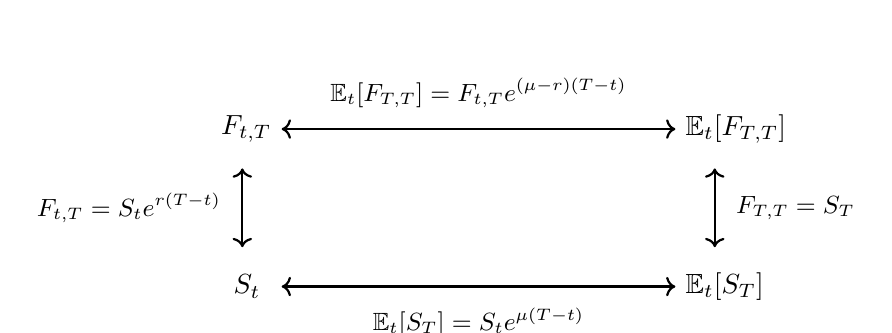
\begin{tikzpicture}
        \draw [<->,thick] (1,0) node [left,xshift=-0.4em]{$S_t$} -- (6,0) node [right]{$\E_t[S_T]$} node [midway,below,yshift=-0.4em]{\small $\E_t[S_T] = S_t e^{\mu(T-t)}$};
        \draw [<->,thick] (1,2) node [left]{$F_{t,T}$} -- (6,2) node [right]{$\E_t[F_{T,T}]$} node [midway,above,yshift=0.4em]{\small $\E_t[F_{T,T}] =F_{t,T} e^{(\mu-r)(T-t)}$};
        \draw [<->,thick] (0.5,0.5) -- (0.5,1.5) node [midway,left,xshift=-0.4em]{\small $F_{t,T}=S_t e^{r(T-t)}$};
        \draw [<->,thick] (6.5,0.5) -- (6.5,1.5) node [midway,right,xshift=0.4em]{\small $F_{T,T}=S_T$};
    \end{tikzpicture}
    \caption{现货期货以及现实测度期望关系}
\end{figure}

\section{看跌-看涨平价关系(欧式期权)}

看跌-看涨期权平价关系(Put-call parity),指具有相同的行权价与到期日的欧式看涨期权与欧式看跌期权,其价格之间存在的关系。若平价关系不成立,则意味着存在套利的空间。现实市场中存在交易成本,又如在中国市场现货无法自由做多做空,因此买卖权平价关系不完全成立。然而欧美市场等流动性较好的市场中,可以近似认为买卖权平价关系成立。

PCP平价可以直接从BS公式中推导;
\begin{align*}
    C_{t,T} &= P_{t,T} + S_t -K \\
    S_t N(d_1) - K e^{-r(T-t)} N(d_2) &= K e^{-r(T-t)} N(-d_2) - S_t N(-d_1) S_t -Ke^{-r(T-t)} \\
    &= K e^{-r(T-t)} [1- N(d_2)] - S_t [1 - N(d_1) ] + S_t -Ke^{-r(T-t)} \\
    &= \cancel{K e^{-r(T-t)}} - K^{-r(T-t)} N(d_2) - \cancel{S_t} + S_t N(d_1) + \cancel{S_t} - \cancel{K^{-r(T-t)}} \\
    &= C_{t,T}
\end{align*}
也可以看到,相同行权价到期时间的看涨看跌期权,两者波动率应该相等,否则PCP平价不成立。


\subsection{无红利资产}

对于无红利资产,使用远期合约(适用于中国市场与美国市场),构建如下两个组合:
\begin{itemize}
    \item 组合A:欧式看涨多头(+C)
    \item 组合B:欧式看跌多头(+P) + \textbf{远期合约}多头(+f)
\end{itemize}

在T时刻,投资组合A与B有:
\begin{table}[ht!]
\centering
\begin{tabular}{ccc}
\toprule
$S_T$与$K$关系 & \multicolumn{1}{c}{投资组合A} & \multicolumn{1}{c}{投资组合B} \\
\midrule
$S_T \geq K$ & $S_T-K$ & $0 + (S_T-K)$ \\
$S_T < K$ & $0$ & $(K - S_T) + (S_T-K)$ \\ 
\bottomrule
\end{tabular}
\end{table}

可以发现在T时刻,两种情况之下A、B两个投资组合的收益相同:
\begin{equation*}
    C(T,S_T) = P(T,S_T) + f(T,S_T)
\end{equation*}

并且根据无套利原则,在任意t时刻两个投资组合的价值也必须相同,否则将存在套利机会:
\begin{equation*}
    C(t,S_t) = P(t,S_t) + f(t,S_t)
\end{equation*}

将远期合约在t时刻价值$f(t,S_t) = S_t - Ke^{-r(T-t)}$代入,则有对于现货价格的PCP公式有:
\begin{equation*}
    C_{t,T} = P_{t,T} +  S_t - K e^{-r(T-t)}
\end{equation*}

利用市场上观察到的看涨看跌期权价格,可求出隐藏现货价格。在中国市场中现货无法做空,可以用期权价格计算隐含现货价格:
\begin{equation*}
    S^*_t = \left( C_{t,T} - P_{t,T} \right) + K e^{-r(T-t)}
\end{equation*}

由于远期价格为$F_{t,T} = S_t e^{r(T-t)}$,可得到对于远期(期货)的PCP公式:
\begin{equation*}
    C_{t,T} = P_{t,T} + \left( F_{t,T} - K \right) e^{-r(T-t)}
\end{equation*}

同样利用市场上已知的看涨看跌期权价格,可求得隐藏期货价格:
\begin{equation*}
    F^*_{t,T} = \left( C_{t,T} - P_{t,T} \right) e^{r(T-t)} + K
\end{equation*}

\subsection{有红利资产}

对于在到期日T之前支付已知红利的标的资产,设支付红利现值为$I_t$,则应有调整后的远期价格为$F_{t,T} = (S_t - I_t)e^{r(T-t)}$,因此调整后的PCP公式有:
\begin{equation*}
    C_{t,T} = P_{t,T} + S_t - I_t - Ke^{-r(T-t)}
\end{equation*}

同理,对于已知红利率资产,设红利率为$q$,调整后的远期价格为$F_{t,T} = S_t e^{(r-q)(T-t)}$,因此有调整后的PCP公式为:
\begin{equation*}
    C_{t,T} = P_{t,T} + S_t e^{-q(T-t)} - Ke^{-r(T-t)}
\end{equation*}

\subsection{中国市场PCP}

在中国市场中,由于标的资产无法自由做多做空,因此现货PCP关系不完全成立。远期可以做多也可以做空,因此远期PCP关系成立:
\begin{equation*}
    C_{t,T} = P_{t,T} + \left( F_{t,T} - K \right) e^{-r(T-t)}
\end{equation*}

目前中国市场中所拥有的金融衍生品与其标的资产如下:
\begin{table}[ht!]
\centering
\begin{tabular}{@{}cccc@{}}
\toprule
\textbf{金融衍生品}    & \textbf{现货}          & \textbf{期货} & \textbf{期权} \\ \midrule
\textbf{股指(中金所)}  &                      & 上证50股指期货    &             \\
\textbf{}         &                      & 沪深300股指期货   & 沪深300股指期权   \\
\textbf{}         &                      & 中证500股指期货   &             \\
\textbf{ETF(上交所)} & 华夏上证50ETF(510050)    &             & 上证50ETF期权   \\
\textbf{}         & 华泰柏瑞沪深300ETF(510300) &             & 沪深300ETF期权  \\
\textbf{ETF(深交所)} & 沪深300ETF(159919)     &             & 沪深300ETF期权  \\ \bottomrule
\end{tabular}
\end{table}

在中国市场中,如上表所示,相同标的的股指期货与期权,或ETF现货与期权之间可以使用PCP关系而不做调整。对于ETF而言,ETF成分股分红,分红会留存在ETF之内。50ETF以及300ETF现货进行分红,期权则会进行相应调整,因此ETF现货与其期权,均受到红利保护,因此不需要调整红利,可视为无红利资产使用PCP关系式。

而对于股指期货而言,指数根据成分股价格加权计算得出,在到期日之内成分股分红,股指将自然回落,不做任何调整,因此股指期货无红利保护。对于沪深300股指期权与股指期货,为同一标的,虽然不受红利保护,但两者之间的PCP也不需要进行调整。可由远期与期权PCP关系计算,如使用股指期权估算隐含远期价格,不需要进行红利调整。

ETF有红利保护,ETF远期(中国市场未上市)无红利保护,因此建立两者之间的PCP关系式则需要调整红利。已知$F_{t,T} = (S_t - I_t)e^{r(T-t)}$,将其代入现货PCP公式可得下列关系式。可理解为由于远期无红利保护,而ETF期权有红利保护,应将远期加上分红,调整为有分红资产:
\begin{equation*}
    C_{t,T} = P_{t,T} + \left( F_{t,T}-K \right) e^{-r(T-t)} + I_t
\end{equation*}

利用如上PCP关系式,则可以使用ETF期权计算出隐藏ETF远期价格:
\begin{equation*}
    F^*_{t,T} = \left( C_{t,T} - P_{t,T} \right) e^{r(T-t)} + K - I_t e^{r(T-t)}
\end{equation*}

\subsection{ETF期权分红调整}

对于股票股利,由于股票稀释,因此需要进行\textbf{除权}(XR,Ex-Right)调整。若配股比例为$25/1000$为1000股配25股,假设拥有1000股的股东,持有股票数目变为$1025$。为了保持公司总市值不变,因此需要进行除权,将市场每股价格等比例下调,做法为将除权日前一天收盘价除以$1+25/1000$。而对于现金股利,则称之为\textbf{除息}(XD,Ex-Dividend)。做法为将除息日前一天的收盘价对应减去现金股利。

交易所之所以会在分红后进行期权合约调整,是因为ETF分红后期权买卖双方的权利义务大小会相应变化。核心的问题是如何通过调整来维持期权合约买卖双方权利义务的均衡。一般来说,期权合约调整有两个目标:
\begin{itemize}
    \item 调整后,合约行权成本(行权价格$\times$合约单位)不变
    \item 调整后,合约市值(结算价格$\times$合约单位)不变
\end{itemize}

\divider

根据《上海证券交易所股票期权试点交易规则》第三章第十三条,对合约标的除权、除息的,期权合约的合约单位、行权价格按照下列公式进行调整:
\small
\begin{equation*}
    \textbf{新合约单位} = \frac{\text{原合约单位}\times\left(1+\text{流通股份实际变动比例}\right)\times\text{除权(息)前一日合约标的收盘价}}{\left(\text{除权(息)前一日合约标的收盘价格}-\text{现金红利}\right)+\text{配股价格}\times\text{流通股份实际变动比例}}
\end{equation*}
\begin{equation*}
    \textbf{新行权价格} = \frac{\text{原行权价格}\times\text{原合约单位}}{\text{新合约单位}}
\end{equation*}
\normalsize

调整后的合约单位,按照四舍五入的原则取整数;调整后的行权价格,按照四舍五入的原则取小数,合约标的为股票的,保留两位小数,合约标的为交易所交易基金的,保留3位小数。

\divider

以华夏上证50ETF为例,根据510050管理人华夏基金2020年11月11日发布《上证50交易型开放式指数证券投资基金利润分配公告》,2020年11月27日为基金分红的权益登记日,11月30日为基金分红的除息日,分红发放日为12月03日,方案为每十份510050基金分红为0.51元,对象为登记日下午交易结束后所有基金份额持有人。根据交易规则,权益登记日下一交易日,即除息日进行除息除权处理。交易所利用前收盘价,计算除权除息参考价格,作为除息日开盘价(集合竞价产生)的参考。在此例子中27日不复权收盘价3.557,前复权收盘价为3.506,为调整了分红后的收盘价(决定涨跌幅)。

上交所于11月11日同日,发布公告将于2020年11月30日对50ETF期权合约的行权价格、合约单位、合约交易代码和合约简称进行调整,并对除息后的50ETF新挂2020年12月、2021年1月、3月和6月等4个月份的标准化合约。已知510050前一个交易日11月27日周五收盘价为3.557元/份,分红金额为每份分红0.051元,流通股份实际变动比例为0,可计算50ETF期权合约的新合约单位为:
\begin{equation*}
    \text{新合约单位} = 10000 \times \frac{3.557}{3.557-0.051} = 10145
\end{equation*}

使用公式计算合约“50ETF购2020年12月3000”新行权价格:
\begin{equation*}
    \text{新行权价格} = \frac{10000}{10145} \times 3.000 = 2.957
\end{equation*}

根据新计算的行权价格,将原合约新挂为“50ETF购2020年12月2957A”。并由于行权价的下调,使得期权买卖双方的权利义务重新平衡。期权合约“50ETF购2020年12月3000”的于27日结算价为0.5616元,由如下公式计算该期权合约30日调整后前结算价(决定保证金):
\begin{equation*}
    \text{新结算价格} = \frac{\text{原结算价格}\times\text{原合约单位}}{\text{新合约单位}} = \frac{10000}{10145} \times 0.5616 = 0.5536
\end{equation*}

可以看到期权合约对于分红的调整有如下几步,先根据ETF27日(除息日30日前一交易日)的收盘价及分红调整合约单位,其实质为缩放比例,为分红调整之后价格与分红之前价格比值的倒数。再根据新合约单位(缩放比例),等比例缩小行权价格与结算价格。合约单位比例放大与价格比例缩小相互抵消,使得合约行权与实际市值保持不变。

\subsubsection*{关于结算价格}

上交所在每个交易日收盘后向市场公布期权合约的结算价格,作为计算期权合约每日日终维持保证金、下一交易日开仓保证金、涨跌停价格等数据的基准。

原则上,期权合约的结算价格为该合约当日收盘集合竞价的成交价格。但是,如果当日收盘集合竞价未形成成交价格,或者成交价格明显不合理,那么上交所就会考虑期权交易的多重影响因素,另行计算合约的结算价格。即根据同标的、同到期日、同类型其他行权价的期权合约隐含波动率,推算该合约隐含波动率,并以此计算该合约结算价。

此外,期权合约最后交易日如果为实值合约的话,由上交所根据合约标的当日收盘价格和该合约行权价格,计算该合约的结算价格;期权合约最后交易日如果为虚值或者平值合约的话,结算价格为0。

期权合约挂牌首日,以上交所公布的开盘参考价作为合约前结算价格。合约标的出现除权、除息的,合约前结算价格按照以下公式进行调整:新合约前结算价格=原合约前结算价格×(原合约单位/新合约单位)。除权除息日,以调整后的合约前结算价作为涨跌幅限制与保证金收取的计算依据。

\section{中国市场特殊处理}

在中国市场存在理论与实务脱节的问题。主要有卖空限制导致现货价格高估,内在价值与时间价值,与平值点定义需要更改。解决同一行权价到期期限的看涨看跌波动率相差大;解决隐含波动率为0;看跌期权时间价值明显高于看涨期权的时间价值;期权时间价值为负;平值点时间价值不是最大等问题。

\textbf{关于无套利与可复制}:无套利指当套利机会出现,人们会利用套利机会获利,使得套利机会消失,表达的是人的主观意愿的假设。而可复制表达是是否能利用套利机会,表达是市场环境是否能允许套利进行。如现货价格被高估,期货价格被低估,虽然人们愿意进行套利,但在中国市场由于现货卖空存在限制,所以难以复制,最终导致了套利无法进行,无套利不满足。

\subsection{做空限制}

在中国市场中,现货市场存在较大的做空限制,使得市场中的价格由所以看多者和少量看空者决定,看空者的情绪无法表达,因此并不能反应所有投资者的真实情绪,现货价格相对被高估。如$F_{t,T}=S_t e^{r(T-t)}$,现货由于卖空限制,难以复制并进行套利。违法BSM假设中允许卖空标的证券的条件,若使用现货价格进入BSM模型存在较大误差。主要解决方法为使用衍生品市场信息代替:
\begin{enumerate}
    \item 继续使用BSM公式,但从衍生品市场提取隐含合理的现货价格:
    \begin{itemize}
        \item 期货中隐含的现货价格(无红利资产):
        \begin{equation*}
            S^*_t = F_{t,T} e^{-r(T-t)}
        \end{equation*}
        \item ETF期权中隐含的现货价格,虽然ETF有红利但期权会进行调整,可视为无红利资产:
        \begin{equation*}
            S^*_t = \left( C_{t,T} - P_{t,T} \right) + Ke^{-r(T-t)}
        \end{equation*}
        \item 股指期权中隐含的现货价格(已知红利率),成分股分行股指不做调整,自然回落:
        \begin{equation*}
            S^*_t = \left( C_{t,T} - P_{t,T} \right)e^{q(T-t)} + Ke^{-(r-q)(T-t)}
        \end{equation*}
    \end{itemize}
    \item 直接使用Black公式,使用期货价格进行计算,即:
    \begin{align*}
        C_{t,T} &= e^{-r(T-t)} \left[ F_{t,T} N(d_1) - K N(d_2) \right] \\
        P_{t,T} &= e^{-r(T-t)} \left[ K N(-d_2) - F_{t,T} N(-d_1) \right]
    \end{align*}
\end{enumerate}

\subsection{内在价值}

已知期权价值可分解为内在价值(Intrinsic value)与时间价值(Time value)两个部分,即:
\begin{equation*}
    \boxed{
        \text{期权价值} = \text{内在价值} + \text{时间价值}
    }
\end{equation*}

以波动划分,内在价值为\textbf{不考虑资产价格波动}的情况下,期权条款赋予期权多头的最高价值。而时间价值为\textbf{标的资产价格波动}为期权多头(权利方)所带来的隐含价值,由于期权的权利方只有权力而无义务,因此期权的内在价值以及时间价值都应大于0。时间价值受内在价值的影响,但内在价值不受时间价值的影响,因而使用两分法。即先计算出期权的内在价值,使用二分法,再确定期权的时间价值。

\subsubsection*{John Hull定义}

定义内在价值为,期权若在当下时点到期,期权所含的的内在价值,如OFOD教科书、上交所、万得中。若美式期权,这样定义就是合理的,由于美式期权在到期日之前可以随时行权,则其内在价值都基于当前时点的股价与行权价进行计算。但如果是欧式期权,则没有考虑行权价货币的时间价值,现货价格为当前时点,但行权价为未来时点,应该对未来时点的行权价进行贴现。且在中国市场由于现货的卖空限制,其实际价格被高估。
\noindent\begin{align*}
    \text{看涨期权内在价值} & = \max(S_t-K,0) \\
    \text{看跌期权内在价值} & = \max(K-S_t,0)
\end{align*}

\subsubsection*{完美市场定义}

在考虑货币时间价值的情形内在价值如下,在完美市场中可适用,但没有考虑中国市场的卖空限制,需要进一步进行调整。
\begin{align*}
    \text{看涨期权内在价值} & = \max\left(S_t-Ke^{-r(T-t)},0\right) \\
    \text{看跌期权内在价值} & = \max\left(Ke^{-r(T-t)}-S_t,0\right)
\end{align*}

\subsubsection*{中国市场定义}

不考虑时间价值,那么欧式看涨权利方与远期合约多头的差别就是期权只有权利而没有义务,因此内在价值应为$\max(f_{t,T},0)$。同理,对于欧式看跌期权应有$\max(-f_{t,T},0)$。即使用期货价格代替现货价格,在期货市场多空双方均能自由表达其看法,且中美市场均可使用,因此有:
\begin{align*}
    \text{看涨期权内在价值} & = \max\left[(F_{t,T}-K)e^{-r(T-t)},0\right] \\
    \text{看跌期权内在价值} & = \max\left[(K-F_{t,T})e^{-r(T-t)},0\right]
\end{align*}

\subsubsection*{ETF期权股指期货定义}

由于在中国市场ETF期权,如50ETF,有红利保护机制。即会下调行权价格,放大每手期权数量,相当于变相抬高了股票价格进行复权,修复由于分红带来的影响,因此可视为无红利资产进行处理。而在中国市场中并没有50ETF期货,只有股指期货,且股指期货不对分红进行调整,即没有红利保护,即其成分股分红后股指自然下跌。因此使用股指期货计算ETF期权内在价值时,还需要再做红利调整。由于在计算期货时将现货中的红利剔除:
\begin{equation*}
    F_{t,T} = ( S_t - I_t )e^{r(T-t)}
\end{equation*}

因此,在计算内在价值时应将剔除的红利加回:
\begin{align*}
    \text{看涨期权内在价值} & = \max\left[ (F_{t,T}-K) e^{-r(T-t)} + I_t \right] \\
    \text{看跌期权内在价值} & = \max\left[ (K-F_{t,T}) e^{-r(T-t)} - I_t \right]
\end{align*}

\subsection{平值点与在值程度}

平值点是使得期权内在价值由正值变化到零(内在价值非负)的临界行权价,因为平值点使得内在价值变为零,则平值点使用远期价格的定义应为$F_{t,T}=K$,这样的定义使得实值虚值部分左右较为对称,利于比较。

同理,对于现货(中国市场使用隐含现货价格)而言,平值点应有:
\begin{itemize}
    \item 无红利:$S_t e^{r(T-t)}$
    \item 有红利:$\left(S_t - I_t \right)e^{r(T-t)} $
    \item 红利率:$S_t e^{(r-q)(T-t)}$
\end{itemize}

使用对数在值程度(Log-moneyness)作为在值程度的定义,优点是使得值域范围有$(-\infty,\infty)$,使得实值期权与虚值期权幅度上对称。
\begin{equation*}
    \ln \frac{K}{K_{\text{ATM}}} = \ln \frac{K}{F}
\end{equation*}

同时可以发现,根据PCP公式:
\begin{equation*}
    C_{t,T} = P_{t,T} + \left( F_{t,T} - K \right) e^{-r(T-t)}
\end{equation*}

根据平值期权ATM定义有$F_{t,T}=K$,易得此时$C_{t,T}=P_{t,T}$。

当$F_{t,T} \geq K$时,此时看涨期权ITM,同时具有内在价值与时间价值。而看跌期权OTM,因此只具有时间价值。由如上定义,此时看涨期权内在价值为$\left( F_{t,T} - K \right) e^{-r(T-t)}$。根据PCP可以看到:
\begin{align*}
    C_{t,T} &= P_{t,T} + \left( F_{t,T} - K \right) e^{-r(T-t)} \\
    \cancel{C_{\text{内在价值}}} + C_{\text{时间价值}}
    &= P_{\text{时间价值}} + \cancel{C_{\text{内在价值}}} \\
    C_{\text{时间价值}} &= P_{\text{时间价值}}
\end{align*}

同理,当$F_{t,T}<K$时,看跌期权为实值,同时具有内在价值与时间价值。因此,在新平值点定义下,\textbf{相同行权价、相同期限的看涨期权与看跌期权的时间价值应该相等}。

\section{平价期权估计}

当平值点为$S_t = K e^{-r(T-t)}$时,将其带入看涨BSM公式当中,则有:
\begin{equation*}
    \frac{C}{S} = N(d_1) - N(d_2)
\end{equation*}

同样,对于看跌期权则有:
\begin{align*}
    \frac{P}{S} & = N(-d_2) - N(-d_1) \\
    & = 1 - N(d_2) - [1-N(d_1)] \\
    & = N(d_1) - N(d_2) = \frac{C}{S}
\end{align*}

对于$d_1$和$d_2$,此时有:
\begin{align*}
    d_1 &= \frac{\ln(S/K)+(r+\sigma^2/2)(T-t)}{\sigma\sqrt{T-t}} = \frac{\sigma}{2}\sqrt{T-t} \\
    d_2 &= \frac{\ln(S/K)+(r-\sigma^2/2)(T-t)}{\sigma\sqrt{T-t}} = d_1 - \sigma\sqrt{T-t}= -\frac{\sigma}{2}\sqrt{T-t}
\end{align*}

则对于欧式平价看涨或看跌期权,有看涨与看跌期权价格相等,将期权价格记为$V$:
\begin{align*}
    \frac{V}{S} &= N \left( \frac{\sigma\sqrt{T-t}}{2} \right) - N\left( -\frac{\sigma\sqrt{T-t}}{2} \right) \\
    & = N \left( \frac{\sigma\sqrt{T-t}}{2} \right) - N\left( -\frac{\sigma\sqrt{T-t}}{2} \right) \\
    & = 2N\left( \frac{\sigma\sqrt{T-t}}{2} \right) - 1
\end{align*}

对于正态分布有CDF:
\begin{equation*}
   N(x) = \int \frac{1}{\sqrt{2\pi}} e^{-\frac{1}{2}x^2} dx
\end{equation*}

已知对于自然指数$e^x$,其泰勒展开有:
\begin{equation*}
    e^x = \sum^{\infty}_{n=0} \frac{x^n}{n!} = 1 + x + \frac{x^2}{2!} + \frac{x^3}{3!} + \dots
\end{equation*}

替换将$x$替换为$-\frac{x^2}{2}$:
\begin{equation*}
    e^{-\frac{x^2}{2}} = 1 -\frac{x^2}{2}  + \frac{x^4}{8} - \frac{x^6}{48} + \dots
\end{equation*}

使用泰勒展开,将正态分布的自然指数替换:
\begin{align*}
   G(x) &= \frac{1}{\sqrt{2\pi}} \int e^{-\frac{x^2}{2}} dx \\
   &= \frac{1}{\sqrt{2\pi}} e^{-\frac{1}{2}} \int \left( 1 -\frac{x^2}{2}  + \frac{x^4}{8} - \frac{x^6}{48} + \dots \right) dx \\
   &= \frac{1}{\sqrt{2\pi}} \left( x -\frac{x^3}{6} + \frac{x^5}{40} - \frac{x^7}{336} + \dots \right) 
\end{align*}

注意在求泰勒展开的积分之后,还需要加上常数项$C$,因此应有:
\begin{equation*}
    N(x) = G(x) + C
\end{equation*}

已知$N(0) = G(0) + C = \frac{1}{2}$,因此$C=\frac{1}{2}$,即:
\begin{equation*}
   N(x) = \frac{1}{2} + \frac{1}{\sqrt{2\pi}} \left( x -\frac{x^3}{6} + \frac{x^5}{40} - \frac{x^7}{336} + \dots \right) 
\end{equation*}

令$x=\frac{\sigma\sqrt{T-t}}{2}$代入上式,则对于欧式平价期权:
\begin{align*}
    \frac{V}{S} & = 2N\left( \frac{\sigma\sqrt{T-t}}{2} \right) - 1 \\
    & = 2\left[\frac{1}{2} + \frac{1}{\sqrt{2\pi}} \left(\frac{\sigma\sqrt{T-t}}{2} - \frac{(\sigma\sqrt{T-t}/2)^3}{6} + \frac{(\sigma\sqrt{T-t}/2)^5}{40} - \dots + \dots\right) \right] - 1\\
    &\approx \frac{\sigma\sqrt{T-t}}{\sqrt{2\pi}} \approx 0.4\sigma\sqrt{T-t}
\end{align*}



\appendix

\begin{appendices}

\section{矩}

\subsection{含义}
数学中矩的概念来自物理学,在物理学中,矩表示距离和物理量的乘积。如力与力臂(参考点的距离)的乘积,得到的是力矩(或扭矩)。可以理解为一杆“秤”,“秤”的平衡的两边重量与距离的乘积相同,则能保持平衡。

而在概率论上,可以理解秤为一杆秤的两端的概率为1,中心点概率为0。如一端秤砣重量,为中奖金额$500$元,但中奖概率为千分之一,即离中心点距离为$0.1\%$,那么期望为$0.5$元。可以理解为了使得秤保持平衡,则另一端,在概率为1,其秤砣重量,中奖金额应为$0.5$元。

\subsection{期望}

这样既可以把期望看成是矩,即距离(概率)乘以力(随机变量)的大小。对于$n$阶矩即对$x^n$q求期望,在离散形式下有:
\begin{equation*}
    E[x] = \sum_i p_i x_i
\end{equation*}

在连续形式下,n阶矩可以表示为$(x-c)^n$的期望,其中$f(x)$为概率密度函数(probability density function):
\begin{equation*}
    \mu_n = \int_{-\infty}^{\infty} (x-c)^n f(x) dx
\end{equation*}

\begin{table}[ht!]
\centering
\begin{tabular}{@{}cll@{}}
\toprule
阶(Order) & \multicolumn{1}{c}{非中心矩(Non-central)} & \multicolumn{1}{c}{中心矩(Central)} \\ \midrule
1st & $\E(x)=\mu $ & \\
2nd & $\E(x^2) $ & $\E[(x-\mu)^2]$   \\
3rd & $\E(x^3) $ & $\E[(x-\mu)^3]$   \\
4th & $\E(x^4) $ & $\E[(x-\mu)^4]$   \\ \bottomrule
\end{tabular}
\end{table}

常用的有一至四阶矩:
\begin{itemize}
    \setlength{\itemsep}{0em}
    \item 均值 $\text{Mean}(x)$ 为一阶中心矩
    \item 方差 $\text{Variance}(x) = \E(x-\mu)^2$ 为二阶非中心矩
    \item 偏度 $\text{Skewness}(x) = \frac{\E[(x-\mu)^4]}{\sigma^3}$ 为三阶标准矩 
    \item 峰度 $\text{Kurtosis}(x) = \frac{\E[(x-\mu)^4]}{\sigma^4}$ 为四阶标准矩
\end{itemize}

\subsection{分类}

\subsubsection*{原点矩(Raw/crude moment)}

当$c=0$时,称为原点矩。此时则有\textbf{平均数(mean)}或\textbf{期望(expected value)}的连续形式为:
\begin{equation*}
    \mu = E(x) = \int_{-\infty}^{\infty} (x-0)^1 f(x) dx =
    \int_{-\infty}^{\infty} x f(x) dx
\end{equation*}

其离散形式为:
\begin{equation*}
    \mu = E(x) = \sum_i x_i p_i
\end{equation*}

\subsubsection*{中心矩(Central moment)}

期望值可以成为随机变量的中心,即当$c=E(x)$时
\begin{equation*}
    \mu_n = E[(x-E(x))^n] = \int_{-\infty}^{\infty} (x-E(x))^n f(x) dx
\end{equation*}

同时可知任何变量的一阶中心矩为0:
\begin{align*}
    \mu_1 &= \int_{-\infty}^{\infty} (x-E(x))^1 f(x) dx \\
    &= \int_{-\infty}^{\infty} x f(x) dx - \int_{-\infty}^{\infty} E(x) f(x) dx \\
    &= E(x) - E(x) \int_{-\infty}^{\infty} f(x) dx \\
    &= E(x) - E(x) \times 1 = 0 
\end{align*}

而二阶中心矩(second central moment)为\textbf{方差(Variance)}
\begin{align*}
    \mu_2 &= \int_{-\infty}^{\infty} (x-E(x))^2 f(x) dx \\
    &= \int_{-\infty}^{\infty} x^2 f(x)dx - 2 E(x) \int_{-\infty}^{\infty} x f(x)dx + [E(x)]^2\int_{-\infty}^{\infty}f(x)dx \\
    &= \int_{-\infty}^{\infty} x^2 f(x)dx - 2 E(x) E(x) + [E(x)]^2\times 1 \\
    &= \int_{-\infty}^{\infty} x^2 f(x)dx - [E(x)]^2 \\
    &= E(x^2) - [E(x)]^2 = \sigma^2
\end{align*}

其离散形式则有:
\begin{equation*}
    \text{Var}(x) = \sigma^2 = \sum p_i (x_i - \mu)^2 
\end{equation*}

\subsubsection*{标准矩(Standardized moment)}

标准矩为标准化(除以标准差)后的中心矩,第$n$阶中心矩(standardized moment of degree n)有:
\begin{equation*}
    \mu_n = E[(x-\mu)^n] = \int_{-\infty}^{\infty} (x-\mu)^n f(x)dx
\end{equation*}

已知标准差的$n$次方有:
\begin{equation*}
    \sigma^n = \left(\sqrt{E[(x-\mu)^2]}\right)^n = (E[(x-\mu^2)])^{n/2}
\end{equation*}

此时,第$n$阶标准矩有:
\begin{equation*}
    \tilde{\mu}_n = \frac{\mu_n}{\sigma^n} = E\left[ \left(\frac{x-\mu}{\sigma}\right)^n \right]
\end{equation*}

由一阶中心矩为$0$,可知一阶标准矩(first standardized moment)也为$0$。而二阶标准矩(second standardized moment)则有:
\begin{equation*}
    \tilde{\mu}_2 = \frac{\mu_2}{\sigma^2} = \frac{E[(x-\mu)^2]}{\left(E[(x-\mu)^2]\right)^{2/2}} = 1
\end{equation*}

\subsubsection*{偏度(skewness)}

三阶标准矩(third standardized moment)为\textbf{偏度}:
\begin{equation*}
    \tilde{\mu}_3 = \frac{\mu_3}{\sigma^3} = \frac{E[(x-\mu)^3]}{\left(E[(x-\mu)^2]\right)^{3/2}}
\end{equation*}

偏度分为两种:
\begin{itemize}
    \item 负偏态或左偏态:左侧的尾部更长,分布的主体集中在右侧
    \item 正偏态或右偏态:右侧的尾部更长,分布的主体集中在左侧
\end{itemize}

\subsubsection*{峰度(kurtosis)}
四阶标准矩(third standardized moment)为\textbf{峰度}:
\begin{equation*}
    \tilde{\mu}_4 = \frac{\mu_4}{\sigma^4} = \frac{E[(x-\mu)^4]}{\left(E[(x-\mu)^2]\right)^{4/2}} 
\end{equation*}

定义\textbf{超值峰度(excess kurtosis)}为峰度$-3$,使得正态分布的峰度为0:
\begin{equation*}
    \text{excess kurtosis} = \tilde{\mu}_4-3
\end{equation*}
\begin{itemize}
    \item 如果超值峰度为正,即峰度值大于3,称为高狭峰(leptokurtic)
    \item 如果超值峰度为负,即峰度值小于3,称为低阔峰(platykurtic)
\end{itemize}

\subsection{矩母函数}

\subsubsection{定义}

矩母函数或称为矩生成函数(Moment generating fuction,MGF)或动差生成函数,顾名思义就是产生矩的函数。对于随机变量$X$,其矩生成函数定义为:
\begin{equation*}
    \boxed{
        M_X(t) = \E(e^{tX})
    }
\end{equation*}

离散形式下有:
\begin{equation*}
    \E[e^{tx}] = \sum e^{tx} P(x)
\end{equation*}

而在连续形势下有:
\begin{equation*}
    \E[e^{tx}] = \int_{-\infty}^{\infty} e^{tx} f(x) dx
\end{equation*}

\begin{thm}
    将矩母函数进行n次求导,并令$t=0$则可得到$\E(X^n)$
    \begin{equation*}
        \E(X^n) = \left. \frac{d^n}{dt^n} M_X(t) \right\vert_{t=0}
    \end{equation*}
\end{thm}

\begin{proof}
    对于$e^x$使用泰勒展开有:
    \begin{equation*}
        e^x = 1 + x + \frac{x^2}{2!} + \frac{x^3}{3!} + \dots + \frac{x^n}{n!}
    \end{equation*}

    那么$e^{tx}$的期望为:
    \begin{align*}
        \E[e^{tx}] &= \E\left[1 + tx + \frac{(tx)^2}{2!} + \frac{(tx)^3}{3!} + \dots + \frac{(tx)^n}{n!} \right] \\
        &= \E(1) + t\E(x) + \frac{t^2}{2!}\E(x^2) + \frac{t^3}{3!}\E(x^3) + \dots + \frac{t^n}{n!}\E(x^n) 
    \end{align*}

    对其求一阶导:
    \begin{align*}
        \frac{d}{dt} \E[e^{tx}] 
        &= \frac{d}{dt} \left[ \E(1) + t\E(x) + \frac{t^2}{2!}\E(x^2) + \frac{t^3}{3!}\E(x^3) + \dots + \frac{t^n}{n!}\E(x^n) \right] \\
        &= 0 + \E(x) + t\E(x^2) + \frac{t^2}{2}\E(x^3) + \dots + \frac{t^{n-1}}{(n-1)!}\E(x^n) \\
        & \qquad \text{(代入$t=0$)} \\
        &= 0 + \E(x) + 0 + 0 + \dots + 0 \\
        &= \E(x) 
    \end{align*}
\end{proof}

\subsubsection{性质}

对于标准正态分布$N\sim(0,1)$的矩母函数,则有:
\begin{align*}
    M_X(t) &= \E (e^{xt}) = \int e^{xt} \frac{1}{\sqrt{\pi}} e^{-\frac{1}{2}x^2}dx \\
    &= \int \frac{1}{\sqrt{\pi}} e^{xt-\frac{1}{2}x^2}dx \\
    &= \int \frac{1}{\sqrt{\pi}} e^{-\frac{1}{2} (x^2 -2xt + t^2 -t^2)}dx \\
    &= \int \frac{1}{\sqrt{\pi}} e^{-\frac{1}{2} (x-t)^2 + \frac{1}{2}t^2}dx \\
    &= e^{\frac{1}{2} t^2} \int \frac{1}{\sqrt{\pi}} e^{-\frac{1}{2} (x-t)^2 }dx \\
    &= e^{\frac{1}{2} t^2}
\end{align*}

对于正态分布$N\sim(\mu,\sigma)$的矩母函数,则有:
\begin{equation*}
    M_X(t) = \E (e^{xt}) = \int e^{xt} \frac{1}{\sigma\sqrt{\pi}} e^{-\frac{1}{2} \left( \frac{x-\mu}{\sigma} \right)} dx
\end{equation*}

此时代换$z=\frac{x-\mu}{\sigma}$,即$x= \sigma z + \mu$,并有$dx=\sigma dz$:
\begin{align*}
    M_X(t) &= \int e^{(\sigma z + \mu)t} \frac{1}{\sigma\sqrt{\pi}} e^{-\frac{1}{2}z^2}dx \\
    &= e^{\mu t} \int e^{\sigma z t} \frac{1}{\sigma\sqrt{\pi}} e^{-\frac{1}{2}z^2}dx \\
    &= e^{\mu t} \int \frac{1}{\sigma\sqrt{\pi}} e^{-\frac{1}{2} (z^2 -2\sigma t z + (\sigma t)^2 -(\sigma t)^2)}dx \\
    &= e^{\mu t} e^{\frac{1}{2} \sigma^2 t^2} \int \frac{1}{\sigma\sqrt{\pi}} e^{-\frac{1}{2} (z - \sigma t)^2}dx \\
    &= e^{\mu t + \frac{1}{2} \sigma^2 t^2}
\end{align*}

\end{appendices}


\end{document}